\documentclass[aspectratio=169,11pt]{beamer}
% ==========================================================================
%  KSA lecture-slide theme  =  stock beamer "Boadilla"  +  KSA colour theme
%  brand colours sampled from the official KSA symbol mark:
%    Deep Prussian Blue  #2E3192   (지성 - intellect)
%    Golden Gray         #D6CBB1   (감성 - sensibility)
%  Engine: XeLaTeX.  Usage:
%    \documentclass[aspectratio=169,11pt]{beamer}
%    % ==========================================================================
%  KSA lecture-slide theme  =  stock beamer "Boadilla"  +  KSA colour theme
%  brand colours sampled from the official KSA symbol mark:
%    Deep Prussian Blue  #2E3192   (지성 - intellect)
%    Golden Gray         #D6CBB1   (감성 - sensibility)
%  Engine: XeLaTeX.  Usage:
%    \documentclass[aspectratio=169,11pt]{beamer}
%    % ==========================================================================
%  KSA lecture-slide theme  =  stock beamer "Boadilla"  +  KSA colour theme
%  brand colours sampled from the official KSA symbol mark:
%    Deep Prussian Blue  #2E3192   (지성 - intellect)
%    Golden Gray         #D6CBB1   (감성 - sensibility)
%  Engine: XeLaTeX.  Usage:
%    \documentclass[aspectratio=169,11pt]{beamer}
%    \input{../theme/ksa-theme.tex}
% ==========================================================================

\usepackage{fontspec}
\usepackage{amsmath,amssymb}
\usepackage{graphicx}
\graphicspath{{figs/}{../figs/}}
\usepackage{booktabs}
\usepackage{listings}

% ---- fonts (no ctex/xeCJK on this box -> fontspec drives CJK directly) -----
\defaultfontfeatures{Ligatures=TeX}
\setmainfont{Noto Sans CJK KR}
\setsansfont{Noto Sans CJK KR}
\setmonofont{Noto Sans Mono CJK KR}[Scale=0.92]

% ---- base theme: stock Boadilla ------------------------------------------
\usetheme{Boadilla}
\usefonttheme{professionalfonts}
\setbeamertemplate{navigation symbols}{}

% ---- KSA colour theme (recolour the stock theme) --------------------------
\definecolor{ksablue}{HTML}{2E3192}
\definecolor{ksabluedk}{HTML}{20226A}
\definecolor{ksagold}{HTML}{D6CBB1}
\definecolor{ksagolddk}{HTML}{A9976B}
\definecolor{ksared}{HTML}{C0392B}
\definecolor{ksagray}{HTML}{5B5B5B}

\setbeamercolor{structure}{fg=ksablue}
\setbeamercolor{alerted text}{fg=ksared}

\setbeamercolor{palette primary}{fg=white,           bg=ksablue}
\setbeamercolor{palette secondary}{fg=white,         bg=ksablue!85!black}
\setbeamercolor{palette tertiary}{fg=white,          bg=ksabluedk}
\setbeamercolor{titlelike}{fg=ksablue}
\setbeamercolor{frametitle}{fg=ksablue,bg=}
\setbeamercolor{title}{fg=ksablue}
\setbeamercolor{author}{fg=ksagray}
\setbeamercolor{institute}{fg=ksagray}
\setbeamercolor{block title}{fg=white,bg=ksablue}
\setbeamercolor{block body}{fg=black!85,bg=ksablue!6}
\setbeamercolor{item}{fg=ksablue}
\setbeamercolor{section in toc}{fg=black!85}

\setbeamerfont{frametitle}{series=\bfseries}
\setbeamerfont{title}{series=\bfseries}

% ---- footline:  KSA mark | "Made by ..." | n / N   (matches reference) ----
\newcommand{\ksacredit}{Made by Sumin Han \,\textperiodcentered\, suminhan@ksa.hs.kr}
\setbeamertemplate{footline}{%
  \hbox{%
    \begin{beamercolorbox}[wd=.18\paperwidth,ht=2.6ex,dp=1.5ex,leftskip=1.1em]{}%
      \raisebox{-0.35ex}{
\includegraphics[height=2.0ex]{ksa-logo.png}}%
    \end{beamercolorbox}%
    \begin{beamercolorbox}[wd=.64\paperwidth,ht=2.6ex,dp=1.5ex,center]{}%
      {\scriptsize\color{ksagray}\ksacredit}%
    \end{beamercolorbox}%
    \begin{beamercolorbox}[wd=.18\paperwidth,ht=2.6ex,dp=1.5ex,rightskip=1.1em]{}%
      \hfill{\scriptsize\color{ksablue}\insertframenumber\,/\,\inserttotalframenumber}%
    \end{beamercolorbox}%
  }%
  \vskip2pt
}

% ---- section divider: stock \sectionpage, KSA-coloured -------------------
\setbeamertemplate{section page}{%
  \begingroup\centering
    {\color{ksagolddk}\rule{0.16\paperwidth}{1pt}}\par\vskip1.0em
    {\usebeamerfont{title}\color{ksablue}\insertsectionhead\par}\vskip1.0em
    {\color{ksagolddk}\rule{0.16\paperwidth}{1pt}}\par
  \endgroup
}
\AtBeginSection[]{\begin{frame}[plain,noframenumbering]\vfill\sectionpage\vfill\end{frame}}

% ---- code listings ------------------------------------------------------------
\lstdefinestyle{ksa}{%
  basicstyle=\ttfamily\scriptsize,
  keywordstyle=\color{ksablue}\bfseries,
  commentstyle=\color{ksagray}\itshape,
  stringstyle=\color{ksagolddk},
  numberstyle=\tiny\color{ksagray},
  backgroundcolor=\color{ksablue!6},
  frame=leftline, framerule=1.4pt, rulecolor=\color{ksablue},
  xleftmargin=1em, aboveskip=0.8em, belowskip=0.4em,
  showstringspaces=false, breaklines=true, language=Python,
}
\lstset{style=ksa}

% ---- handy macros -----------------------------------------------------------
\newcommand{\kb}[1]{\textbf{\color{ksablue}#1}}   % blue keyword
\newcommand{\kq}[1]{\textbf{\color{ksared}#1}}    % red key-question

% ==========================================================================

\usepackage{fontspec}
\usepackage{amsmath,amssymb}
\usepackage{graphicx}
\graphicspath{{figs/}{../figs/}}
\usepackage{booktabs}
\usepackage{listings}

% ---- fonts (no ctex/xeCJK on this box -> fontspec drives CJK directly) -----
\defaultfontfeatures{Ligatures=TeX}
\setmainfont{Noto Sans CJK KR}
\setsansfont{Noto Sans CJK KR}
\setmonofont{Noto Sans Mono CJK KR}[Scale=0.92]

% ---- base theme: stock Boadilla ------------------------------------------
\usetheme{Boadilla}
\usefonttheme{professionalfonts}
\setbeamertemplate{navigation symbols}{}

% ---- KSA colour theme (recolour the stock theme) --------------------------
\definecolor{ksablue}{HTML}{2E3192}
\definecolor{ksabluedk}{HTML}{20226A}
\definecolor{ksagold}{HTML}{D6CBB1}
\definecolor{ksagolddk}{HTML}{A9976B}
\definecolor{ksared}{HTML}{C0392B}
\definecolor{ksagray}{HTML}{5B5B5B}

\setbeamercolor{structure}{fg=ksablue}
\setbeamercolor{alerted text}{fg=ksared}

\setbeamercolor{palette primary}{fg=white,           bg=ksablue}
\setbeamercolor{palette secondary}{fg=white,         bg=ksablue!85!black}
\setbeamercolor{palette tertiary}{fg=white,          bg=ksabluedk}
\setbeamercolor{titlelike}{fg=ksablue}
\setbeamercolor{frametitle}{fg=ksablue,bg=}
\setbeamercolor{title}{fg=ksablue}
\setbeamercolor{author}{fg=ksagray}
\setbeamercolor{institute}{fg=ksagray}
\setbeamercolor{block title}{fg=white,bg=ksablue}
\setbeamercolor{block body}{fg=black!85,bg=ksablue!6}
\setbeamercolor{item}{fg=ksablue}
\setbeamercolor{section in toc}{fg=black!85}

\setbeamerfont{frametitle}{series=\bfseries}
\setbeamerfont{title}{series=\bfseries}

% ---- footline:  KSA mark | "Made by ..." | n / N   (matches reference) ----
\newcommand{\ksacredit}{Made by Sumin Han \,\textperiodcentered\, suminhan@ksa.hs.kr}
\setbeamertemplate{footline}{%
  \hbox{%
    \begin{beamercolorbox}[wd=.18\paperwidth,ht=2.6ex,dp=1.5ex,leftskip=1.1em]{}%
      \raisebox{-0.35ex}{
\includegraphics[height=2.0ex]{ksa-logo.png}}%
    \end{beamercolorbox}%
    \begin{beamercolorbox}[wd=.64\paperwidth,ht=2.6ex,dp=1.5ex,center]{}%
      {\scriptsize\color{ksagray}\ksacredit}%
    \end{beamercolorbox}%
    \begin{beamercolorbox}[wd=.18\paperwidth,ht=2.6ex,dp=1.5ex,rightskip=1.1em]{}%
      \hfill{\scriptsize\color{ksablue}\insertframenumber\,/\,\inserttotalframenumber}%
    \end{beamercolorbox}%
  }%
  \vskip2pt
}

% ---- section divider: stock \sectionpage, KSA-coloured -------------------
\setbeamertemplate{section page}{%
  \begingroup\centering
    {\color{ksagolddk}\rule{0.16\paperwidth}{1pt}}\par\vskip1.0em
    {\usebeamerfont{title}\color{ksablue}\insertsectionhead\par}\vskip1.0em
    {\color{ksagolddk}\rule{0.16\paperwidth}{1pt}}\par
  \endgroup
}
\AtBeginSection[]{\begin{frame}[plain,noframenumbering]\vfill\sectionpage\vfill\end{frame}}

% ---- code listings ------------------------------------------------------------
\lstdefinestyle{ksa}{%
  basicstyle=\ttfamily\scriptsize,
  keywordstyle=\color{ksablue}\bfseries,
  commentstyle=\color{ksagray}\itshape,
  stringstyle=\color{ksagolddk},
  numberstyle=\tiny\color{ksagray},
  backgroundcolor=\color{ksablue!6},
  frame=leftline, framerule=1.4pt, rulecolor=\color{ksablue},
  xleftmargin=1em, aboveskip=0.8em, belowskip=0.4em,
  showstringspaces=false, breaklines=true, language=Python,
}
\lstset{style=ksa}

% ---- handy macros -----------------------------------------------------------
\newcommand{\kb}[1]{\textbf{\color{ksablue}#1}}   % blue keyword
\newcommand{\kq}[1]{\textbf{\color{ksared}#1}}    % red key-question

% ==========================================================================

\usepackage{fontspec}
\usepackage{amsmath,amssymb}
\usepackage{graphicx}
\graphicspath{{figs/}{../figs/}}
\usepackage{booktabs}
\usepackage{listings}

% ---- fonts (no ctex/xeCJK on this box -> fontspec drives CJK directly) -----
\defaultfontfeatures{Ligatures=TeX}
\setmainfont{Noto Sans CJK KR}
\setsansfont{Noto Sans CJK KR}
\setmonofont{Noto Sans Mono CJK KR}[Scale=0.92]

% ---- base theme: stock Boadilla ------------------------------------------
\usetheme{Boadilla}
\usefonttheme{professionalfonts}
\setbeamertemplate{navigation symbols}{}

% ---- KSA colour theme (recolour the stock theme) --------------------------
\definecolor{ksablue}{HTML}{2E3192}
\definecolor{ksabluedk}{HTML}{20226A}
\definecolor{ksagold}{HTML}{D6CBB1}
\definecolor{ksagolddk}{HTML}{A9976B}
\definecolor{ksared}{HTML}{C0392B}
\definecolor{ksagray}{HTML}{5B5B5B}

\setbeamercolor{structure}{fg=ksablue}
\setbeamercolor{alerted text}{fg=ksared}

\setbeamercolor{palette primary}{fg=white,           bg=ksablue}
\setbeamercolor{palette secondary}{fg=white,         bg=ksablue!85!black}
\setbeamercolor{palette tertiary}{fg=white,          bg=ksabluedk}
\setbeamercolor{titlelike}{fg=ksablue}
\setbeamercolor{frametitle}{fg=ksablue,bg=}
\setbeamercolor{title}{fg=ksablue}
\setbeamercolor{author}{fg=ksagray}
\setbeamercolor{institute}{fg=ksagray}
\setbeamercolor{block title}{fg=white,bg=ksablue}
\setbeamercolor{block body}{fg=black!85,bg=ksablue!6}
\setbeamercolor{item}{fg=ksablue}
\setbeamercolor{section in toc}{fg=black!85}

\setbeamerfont{frametitle}{series=\bfseries}
\setbeamerfont{title}{series=\bfseries}

% ---- footline:  KSA mark | "Made by ..." | n / N   (matches reference) ----
\newcommand{\ksacredit}{Made by Sumin Han \,\textperiodcentered\, suminhan@ksa.hs.kr}
\setbeamertemplate{footline}{%
  \hbox{%
    \begin{beamercolorbox}[wd=.18\paperwidth,ht=2.6ex,dp=1.5ex,leftskip=1.1em]{}%
      \raisebox{-0.35ex}{
\includegraphics[height=2.0ex]{ksa-logo.png}}%
    \end{beamercolorbox}%
    \begin{beamercolorbox}[wd=.64\paperwidth,ht=2.6ex,dp=1.5ex,center]{}%
      {\scriptsize\color{ksagray}\ksacredit}%
    \end{beamercolorbox}%
    \begin{beamercolorbox}[wd=.18\paperwidth,ht=2.6ex,dp=1.5ex,rightskip=1.1em]{}%
      \hfill{\scriptsize\color{ksablue}\insertframenumber\,/\,\inserttotalframenumber}%
    \end{beamercolorbox}%
  }%
  \vskip2pt
}

% ---- section divider: stock \sectionpage, KSA-coloured -------------------
\setbeamertemplate{section page}{%
  \begingroup\centering
    {\color{ksagolddk}\rule{0.16\paperwidth}{1pt}}\par\vskip1.0em
    {\usebeamerfont{title}\color{ksablue}\insertsectionhead\par}\vskip1.0em
    {\color{ksagolddk}\rule{0.16\paperwidth}{1pt}}\par
  \endgroup
}
\AtBeginSection[]{\begin{frame}[plain,noframenumbering]\vfill\sectionpage\vfill\end{frame}}

% ---- code listings ------------------------------------------------------------
\lstdefinestyle{ksa}{%
  basicstyle=\ttfamily\scriptsize,
  keywordstyle=\color{ksablue}\bfseries,
  commentstyle=\color{ksagray}\itshape,
  stringstyle=\color{ksagolddk},
  numberstyle=\tiny\color{ksagray},
  backgroundcolor=\color{ksablue!6},
  frame=leftline, framerule=1.4pt, rulecolor=\color{ksablue},
  xleftmargin=1em, aboveskip=0.8em, belowskip=0.4em,
  showstringspaces=false, breaklines=true, language=Python,
}
\lstset{style=ksa}

% ---- handy macros -----------------------------------------------------------
\newcommand{\kb}[1]{\textbf{\color{ksablue}#1}}   % blue keyword
\newcommand{\kq}[1]{\textbf{\color{ksared}#1}}    % red key-question


\title{동적계획법 (Dynamic Programming)}
\subtitle{벨만 최적방정식과 정책평가 · 정책 반복과 GridWorld 실습 · 가치 반복, 수렴 증명, 모델 기반의 전제}
\author{Machine Learning 2 \,\textperiodcentered\, 4주차}
\institute{한국과학영재학교 (KSA)}
\date{Chapter 4}

\begin{document}

% ===== title =====
\begin{frame}[plain,noframenumbering]\titlepage\end{frame}

% ===== overview =====
\begin{frame}{이번 주차 개요}
  \begin{columns}[T]
    \begin{column}{0.58\textwidth}
      Chapter 3에서 MDP를 정식화했지만, ``무한히 먼 미래까지
      내다보아야 하는 것처럼 보이는'' 누적 보상 최대화 문제는
      여전히 \textbf{계산 불가능}해 보인다. 벨만의 통찰은 이 무한합을
      \kb{재귀적 관계}로 다시 쓸 수 있다는 것(3.3절 벨만 기대방정식).
      이번 장은 그 재귀식을 \textbf{실제로 계산하는 절차}를 다룬다.
      \vskip0.4em
      \begin{block}{이 챕터를 마치면}
        \begin{itemize}
          \item 벨만 기대방정식으로 주어진 정책의 $V^\pi, Q^\pi$ 를
            \kb{반복적 정책평가}로 계산한다.
          \item 정책 반복의 두 단계가 왜 필요하고, \kb{``멈추면
            최적''}인지를 정책개선 정리(단조 증가) + 유한성으로
            설명한다.
          \item 가치 반복(평가 한 번 + 바로 개선)을 비교하고,
            \kb{축소 사상(바나흐 고정점 정리)}이 수렴을 보장함을
            설명한다.
          \item \kb{모델 기반}($P$ 를 정확히 아는) 전제의 한계를
            짚고, model-free(Ch.\,5--6)의 필요성을 예측한다.
        \end{itemize}
      \end{block}
    \end{column}
    \begin{column}{0.42\textwidth}
      \textbf{세 차시} (5칸 GridWorld 위에서 직관이 쌓인다)
      \begin{enumerate}
        \item \kb{4.1 벨만 최적방정식과 정책평가}
          \,\--- 연립방정식 직접 풀이 vs 반복, $V^\pi$/$Q^\pi$ 다리,
          최적방정식 유도.
        \item \kb{4.2 정책 반복과 GridWorld 실습}
          \,\--- 평가$\to$개선을 GridWorld에서 돌리고 ``멈추면
          최적''을 정리로, 수정된 정책 반복까지.
        \item \kb{4.3 가치 반복, 수렴 증명, 모델 기반 전제}
          \,\--- ``한 줄 차이''인 가치 반복, $k$스텝 내다보기,
          바나흐 고정점 정리, 전제 한계.
      \end{enumerate}
      \vskip0.5em
      {\footnotesize 한 줄 감각: 벨만방정식은 \textbf{연립방정식이
      아니라 반복 대입으로 푸는 것}. 이 감각은 Ch.\,6 TD(경험으로
      근사)와 Ch.\,9 DQN(신경망으로 고정점 찾기)까지 그대로
      재사용된다.}
    \end{column}
  \end{columns}
\end{frame}

\section{4.1 벨만 최적방정식과 정책평가}

\begin{frame}{이 절에서 무엇을 만들 것인가}
  이 절은 세 가지를 만든다.
  \begin{enumerate}
    \item 3.3절의 \kb{벨만 기대방정식}을 ``풀기 위한 도구''로
      다시 읽는 법 --- \kb{벨만 연산자} $T^\pi$ 로.
    \item 3-state 순환 MDP를 \textbf{반복 없이}(연립 일차방정식
      직접 풀이)와 \textbf{반복으로}(정책평가) 두 길로 풀어
      비교해, ``같은 고정점의 다른 길''임을 체감.
    \item $V^\pi$ 와 \kb{$Q^\pi$} 사이의 다리 $Q^\pi(s,\pi(s)) =
      V^\pi(s)$ 와, 여기에 $\max$ 를 넣은 \kb{벨만 최적방정식}.
  \end{enumerate}
  \vskip0.8em
  {\footnotesize 4.2·4.3절의 모든 알고리즘은 4.1절의 이 세 가지
  (연산자 반복 · $Q^\pi$ 점수표 · $\max$)의 조합일 뿐이다.}
\end{frame}

\begin{frame}{복습: 벨만 기대방정식과 \kb{벨만 연산자} $T^\pi$}
  \kb{결정론적 정책}(각 상태에서 정확히 한 행동 $\pi(s)$)로 쓰면:
  \[
  V^\pi(s) = R(s, \pi(s)) + \gamma \sum_{s'} P(s'|s,\pi(s)) V^\pi(s')
  \]
  직관: ``지금 상태의 가치 = 지금 당장 받는 보상 + 할인된 다음
  상태들의 가치의 기댓값.'' --- 게임이 끝날 때까지 통째로 계산
  대신, \textbf{한 스텝 앞만 내다보는 계산을 반복}하면 정확한
  답에 도달한다.
  \vskip0.4em
  확률적 정책 일반형 $\pi(a|s)$ 로 쓰면 우변이 \textbf{가중합}:
  \[
  V^\pi(s) = \sum_a \pi(a|s)\Big[R(s,a)
  + \gamma \sum_{s'} P(s'|s,a)\, V^\pi(s')\Big]
  \]
  이 전체를 \kb{벨만 연산자} $T^\pi$ (``가치함수를 먹여 우변을
  돌려주는 함수의 함수'')라 부른다. 모든 반복법은 \textbf{이
  연산자를 같은 값에 계속 대입}:
  \[
  V_0 \xrightarrow{T^\pi} V_1 \xrightarrow{T^\pi} \cdots
  \xrightarrow{T^\pi} V^\pi
  \]
  이 관점이 4.3절 ``왜 수렴하는가'' 증명의 핵심.
\end{frame}

\begin{frame}{$V^\pi$ 와 $Q^\pi$: 동전의 양면, 그리고 2$\times$2}
  \kb{행동가치함수} $Q^\pi(s,a)$ --- ``상태 $s$ 에서 \textbf{행동
  $a$ 를 강제 한 번 취하고}, 그 다음부터 $\pi$ 를 따른다''의
  가치 --- 는 $V^\pi$ 와 같은 방식으로 재귀되고, 다리
  $Q^\pi(s,\pi(s)) = V^\pi(s)$ 로 서로를 정의하는 \kb{동전의
  양면}:
  \[
  Q^\pi(s,a) = R(s,a) + \gamma \sum_{s'} P(s'|s,a)\, V^\pi(s')
  \]
  \begin{columns}[T]
    \begin{column}{0.44\textwidth}
      \centering
      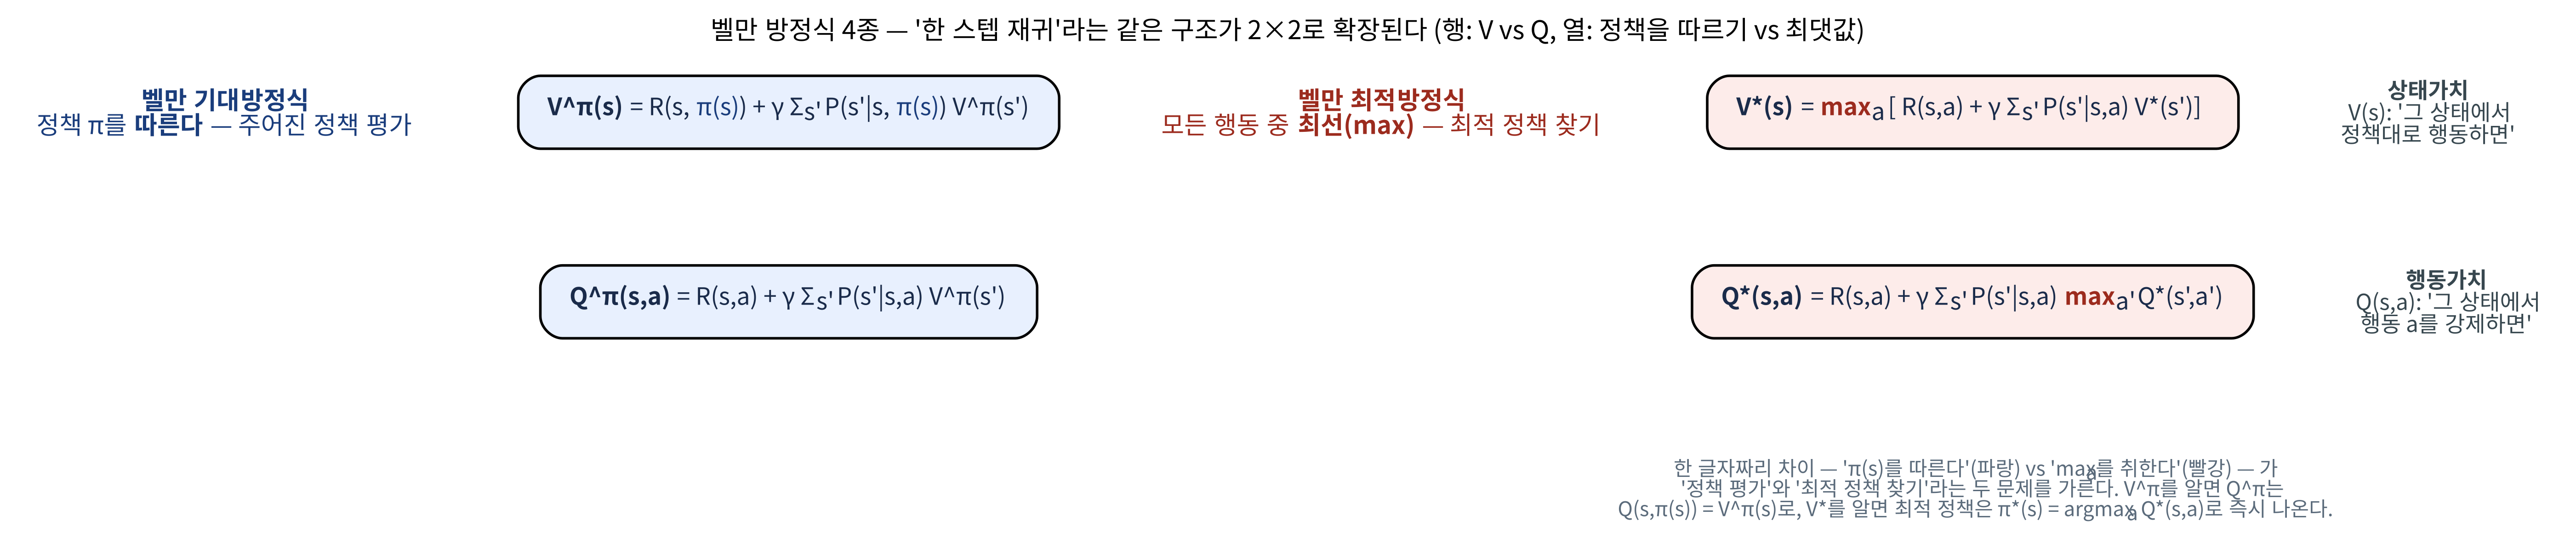
\includegraphics[width=0.95\linewidth]{ch04_1_bellman_equations.png}
      \vskip0.3em
      {\footnotesize 네 개의 벨만방정식: \textbf{기대 vs
      최적} × \textbf{$V$ vs $Q$} 로 2$\times$2.}
    \end{column}
    \begin{column}{0.56\textwidth}
      \small
      \begin{tabular}{@{}lcc@{}}
        \toprule
         & \kb{기대}($\pi$ 를 따른다) & \kb{최적}($\max$) \\
        \midrule
        \textbf{$V$} & $V^\pi$ (4.1절 = 오늘) & $V^{*}$ (4.2--4.3절) \\
        \textbf{$Q$} & $Q^\pi$ & $Q^{*}$ (Ch.\,9 DQN) \\
        \bottomrule
      \end{tabular}
      \vskip0.4em
      {\footnotesize 이번 절의 모든 코드와 수식이 이 다리(V-방정식
      $\leftrightarrow$ Q-방정식 사이)를 통해 오간다.}
    \end{column}
  \end{columns}
\end{frame}

\begin{frame}[fragile]{실습 (1/3): 3-state 순환 MDP를 두 길로}
  ``연립 일차방정식''을 직접 만진다. 3.3절 2상태 왕복 예(행동
  1개)를 \textbf{확률적 전이} 3상태 버전으로 ($\gamma = 0.9$):
  상태 0: $+1$, \textbf{항상} 1로. 상태 1: $+2$, 2로 0.7 / 0으로
  0.3. 상태 2: $0$, \textbf{항상} 0으로. 행동을 하나뿐이므로
  정책은 자명 --- \kq{평가할 것: 상태 0·1·2의 가치?}
\begin{lstlisting}
P = {0: {0: [(1.0, 1)]},
     1: {0: [(0.7, 2), (0.3, 0)]},
     2: {0: [(1.0, 0)]}}
R = {0: {0: 1.0}, 1: {0: 2.0}, 2: {0: 0.0}}
policy = [0, 0, 0];  gamma = 0.9
\end{lstlisting}
  \textbf{방법 1 (연립방정식 직접 풀이)}: 세 방정식
  $V(0) = 1 + 0.9\,V(1)$,
  $V(1) = 2 + 0.9\,(0.7\,V(2) + 0.3\,V(0))$,
  $V(2) = 0.9 V(0)$ 를 대입·정리하면
  $0.2467\,V(0) = 2.8$ $\Rightarrow$ $V(0) \approx 11.3498$,
  $V(1) \approx 11.4998$, $V(2) \approx 10.2148$.
  (검산: $1 + 0.9 \times 11.4998 \approx 11.3498$ $\checkmark$.
  Ch.\,2.2 정규방정식과 같은 가족.)
\end{frame}

\begin{frame}{실습 (2/3): 방법 2 --- 반복적 대입(sweep)}
  같은 값을 \textbf{직접 풀지 않고} 반복법으로. $V$ 를 0으로
  시작해 0$\to$1$\to$2 순서로 \textbf{in-place} 한 스텝씩 갱신:
  \small
  \begin{tabular}{@{}rrrrl@{}}
    \toprule
    sweep & $V(0)$ & $V(1)$ & $V(2)$ & 최대 변화 $\Delta$ \\
    \midrule
    1 & 1.0000 & 2.2700 & 0.9000 & 2.2700 \\
    2 & 3.0430 & 3.3886 & 2.7387 & 2.0430 \\
    3 & 4.0497 & 4.8188 & 3.6448 & 1.4302 \\
    5 & 6.1635 & 6.6902 & 5.5471 & 0.9530 \\
    7 & 7.6514 & 8.0469 & 6.8862 & 0.6565 \\
    $\vdots$ & $\vdots$ & $\vdots$ & $\vdots$ & ($\approx \times 0.9$씩) \\
    \textbf{88} & \textbf{11.3498} & \textbf{11.4998} & \textbf{10.2148} & $< 10^{-6}$ $\to$ 종료 \\
    \bottomrule
  \end{tabular}
  \vskip0.8em
  \begin{block}{확인할 것}
    \textbf{88회} sweep을 거치고 나서야 $\Delta < 10^{-6}$ ---
    방법 1과 \textbf{같은 값}$(11.3498, 11.4998, 10.2148)$.
    두 방법은 ``\kb{같은 고정점을 찾는 다른 길}''이다.
  \end{block}
\end{frame}

\begin{frame}{실습 (3/3): 이 예가 보여주는 세 가지}
  \begin{enumerate}
    \item \kb{``연립방정식''의 실질.} ``벨만방정식을 풀다'' =
      $n$개 미지수 $V(s)$ 에 대한 $n$개 일차방정식. 3개면
      손으로, 100개면 $100 \times 100$ 역산(귀찮지만 가능),
      100만 개면 \textbf{사실상 불가능}.
    \item \kb{수렴은 ``느리다''가 정석.} 오류가 sweep마다 대략
      $\times \gamma$ 배. $\gamma = 0.9$ 이면 절반까지
      $\approx 6.6$회, $10^{-6}$ 까지 $\approx 120$회.
      $\gamma = 0.99$ 라면 ``수백$\sim$수천 sweep''.
    \item \kb{수렴은 초기값에 무관.} 0으로 시작해도
      $V = [100, -50, 10]$ 처럼 아무렇게나 잡아도 \textbf{같은}
      $V^\pi$ 로 수렴(4.3절 바나흐 고정점 정리).
  \end{enumerate}
  {\footnotesize 이 반복적 정책평가는 Sutton·Barto(2018) 표준
  교과서 4장 ``Dynamic Programming''과 동일. 4.3절 연습 2의
  \textbf{비순환} MDP는 ``터미널부터 거꾸로 대입''만으로 답이
  나오는 특수 경우.}
\end{frame}

\begin{frame}[fragile]{반복적 정책평가: 코드}
  상태가 많으면 다음을 값이 더 이상 안 바뀔 때까지 반복 근사:
\begin{lstlisting}
def policy_evaluation(P, R, policy, gamma, theta=1e-6):
    n_states = len(P)
    V = [0.0] * n_states
    while True:
        delta = 0                     # 매 sweep 시작마다 초기화!
        for s in range(n_states):
            a = policy[s]
            v_new = R[s][a] + gamma * sum(prob * V[next_s]
                                          for prob, next_s in P[s][a])
            delta = max(delta, abs(v_new - V[s]))
            V[s] = v_new             # in-place: 갱신된 값을 즉시 사용
        if delta < theta:
            break
    return V
\end{lstlisting}
  \vskip0.2em
  매 sweep마다 모든 상태의 $V(s)$ 를 벨만 우변으로 갱신. 우변의
  $V(s')$ 는 아직 \textbf{정확한 값이 아닌} 추정치인데도,
  $\gamma < 1$ 이면 정확한 $V^\pi$ 로 수렴(\kb{수축 사상},
  4.3절 증명).
\end{frame}

\begin{frame}{in-place(가우시) vs synchronous(야코비)}
  \begin{columns}[T]
    \begin{column}{0.5\textwidth}
      \kb{in-place (가우시)} --- 위 코드
      \begin{itemize}
        \item sweep \textbf{안에서도}, 앞쪽 상태가 갱신된 값을
          뒤쪽이 \textbf{즉시} 사용.
        \item sweep 중반 $V$ 는 ``어떤'' 가치함수의 우변도
          아니지만, $\gamma < 1$ 이면 같은 고정점으로 수렴.
      \end{itemize}
    \end{column}
    \begin{column}{0.5\textwidth}
      \kb{synchronous (야코비)}
      \begin{itemize}
        \item sweep을 \textbf{완전히 끝낸 뒤}에야 갱신
          ($V$ 는 이전 sweep의 값).
        \item $V_{\text{new}}$ 리스트를 따로 모았다가 교체.
      \end{itemize}
    \end{column}
  \end{columns}
  \vskip0.6em
  \begin{block}{실용적 차이}
    둘 다 \textbf{같은 답}에 수렴하지만 \textbf{속도}는 다를 수
    있다. sweep당 비용은 동일하고, in-place가 갱신 정보가 sweep
    안에 전파돼 보통 \textbf{2$\sim$10배} sweep 수를 아낀다.
  \end{block}
\end{frame}

\begin{frame}{``정보의 전파''로 보는 수렴}
  \kq{``왜 우변에 아직 안 푼 값이 들어가도 될까?''}
  \vskip0.5em
  답은 \kb{전파(propagation)} 직관. 5칸 GridWorld(칸 4가 목표,
  걸음마다 $-1$, $\gamma = 0.9$)에서 ``오른쪽'' 정책을 평가하면:
  sweep 1에서 ``목표가 가까울수록 $-1$''이라는 \textbf{약간
  정확한} 정보가 퍼지고, sweep 2에서 \textbf{한 칸 더} 왼쪽으로
  이동, 계속되면 $-1 - 0.9 - 0.9^2 - \cdots$ 의 꼬리 합으로
  수렴.
  \vskip0.5em
  \begin{block}{경험칙}
    \textbf{``정보는 한 sweep에 한 칸 전파된다.''} $\Rightarrow$
    sweep 수 $\approx$ 목표까지 최대 거리 $\times$ (할인이
    충분히 작아질 때까지의 횟수). \textbf{순환} MDP에서는
    ``순환 한 바퀴 전파''.
  \end{block}
  {\footnotesize \textbf{손으로 한 sweep}: ``왼쪽'' 정책을 0에서
  시작해 in-place로 돌리면 sweep 1 $\to$
  $[-1.0000, -1.9000, -2.7100, -3.4390, 0]$, sweep 2 $\to$
  $[-1.9000, -2.7100, \ldots]$ --- 첫 sweep에서 $-1$ 이 한 칸,
  두 번째에서 $-1.9 = -1 + 0.9 \times (-1)$ 이 한 칸 전파.
  수렴값 $-10$ 은 $\sum_{k=0}^{\infty} (-1)(0.9)^k
  = \frac{-1}{1-0.9} = -10$ --- 벽에 막혀 왼쪽으로 밀리는
  \textbf{무한 루프}의 가치(약 133 sweep).}
\end{frame}

\begin{frame}{두 정책 나란히: ``왼쪽''의 나쁨을 정량화}
  ``왼쪽'' 정책은 이 GridWorld에서 \textbf{나쁜 정책}이지만,
  그 ``나쁨''을 정량화하는 것이 $V^{\text{left}}(s) = -10$.
  \vskip0.4em
  \begin{columns}[T]
    \begin{column}{0.44\textwidth}
      \centering
      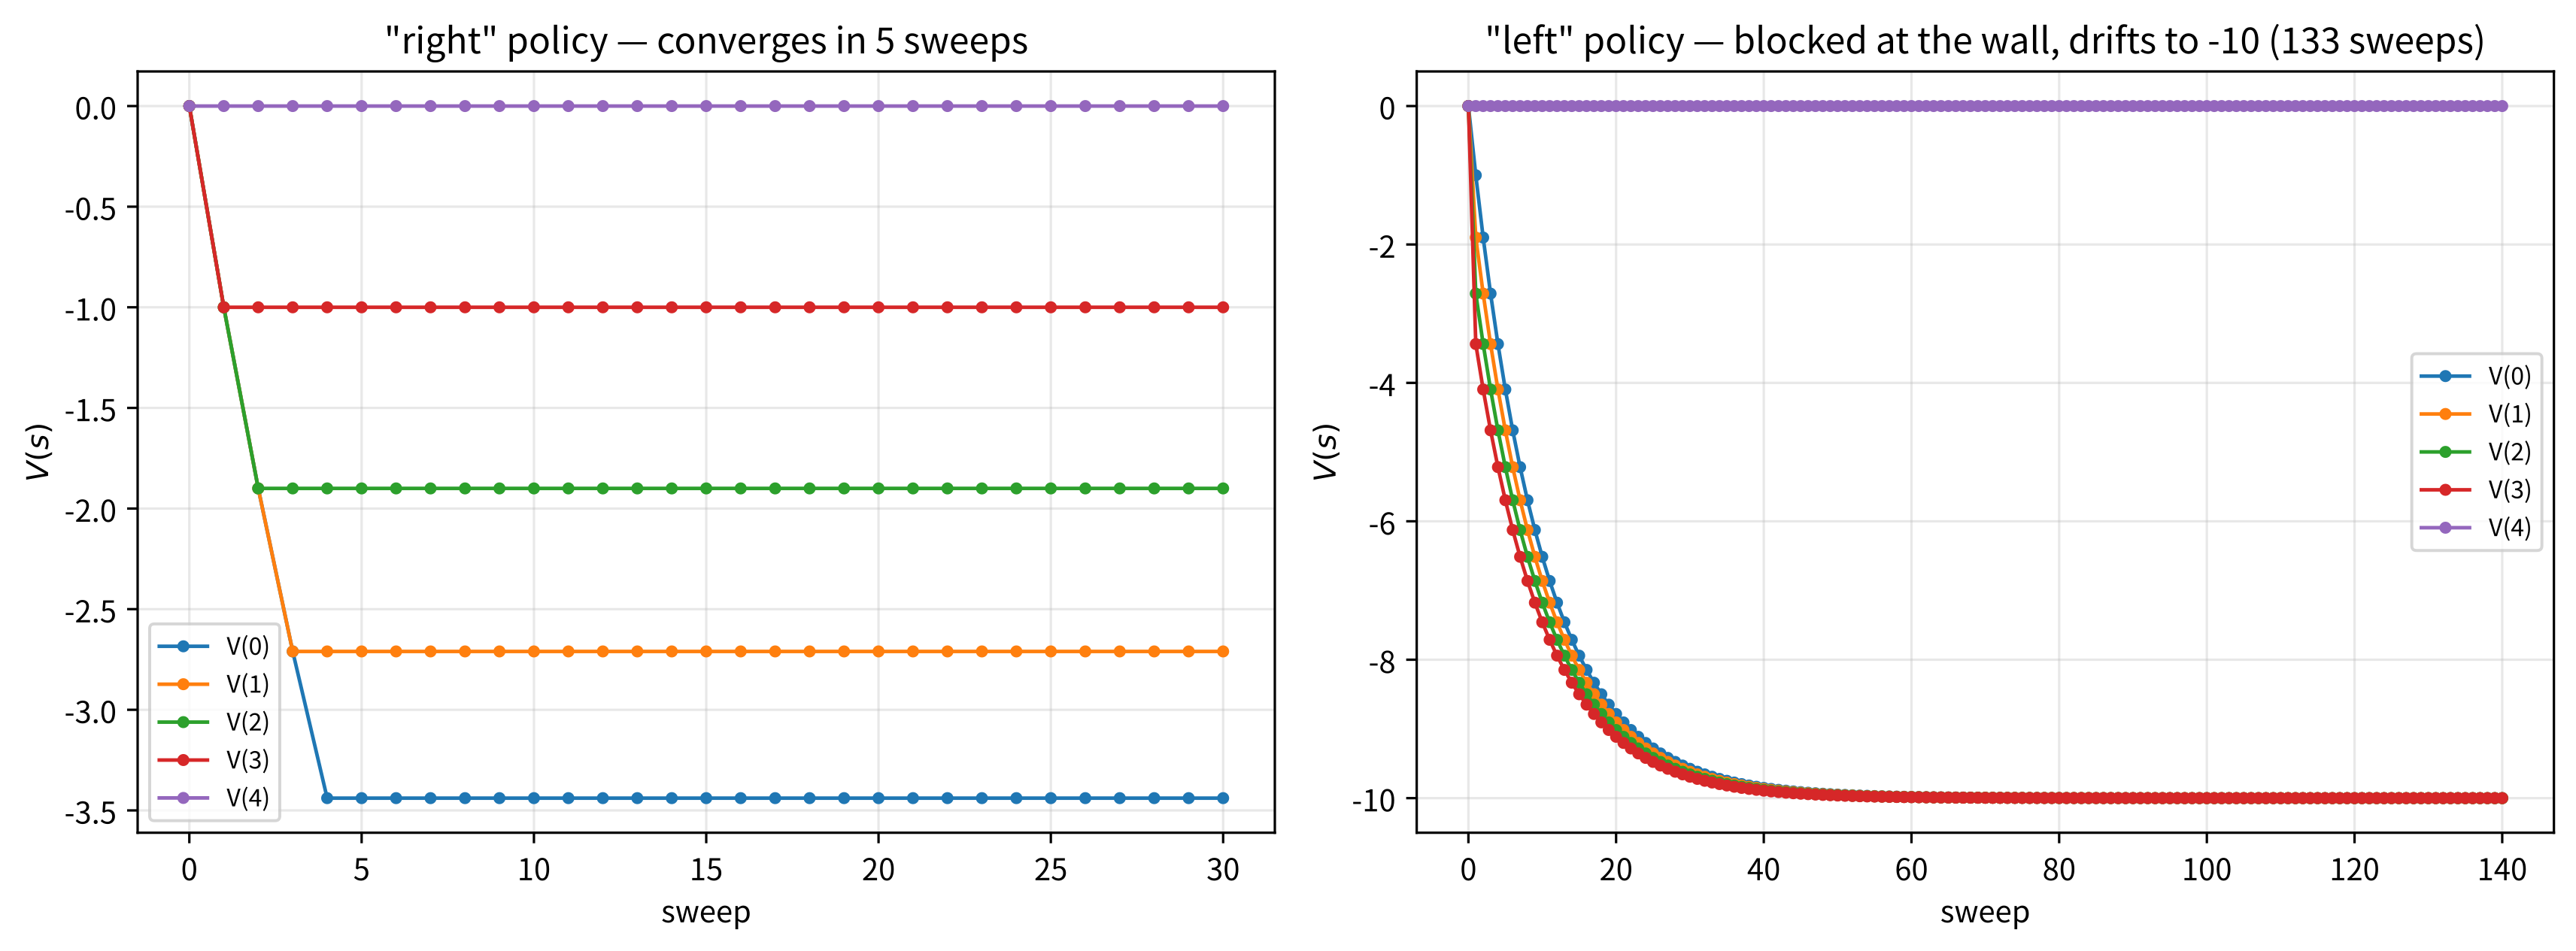
\includegraphics[width=\linewidth]{ch04_1_policy_evaluation_convergence.png}
      \vskip0.3em
      {\footnotesize 두 정책의 반복적 정책평가 수렴 곡선
      ($V(0)$, in-place sweep 단위).}
    \end{column}
    \begin{column}{0.54\textwidth}
      {\small
      \begin{tabular}{@{}lr@{}}
        \toprule
        & $V$ \\
        \midrule
        right & $[-3.439, -2.710, -1.900, -1.000, 0]$ \\
        left & $[-10.000, -10.000, -10.000, -10.000, 0]$ \\
        \bottomrule
      \end{tabular}}
      \vskip0.5em
      \begin{itemize}
        \item ``오른쪽''은 \textbf{5 sweep} 만에 수렴 --- 4.2절
          ``정책 반복이 첫 sweep에서 멈춘다''와 일치.
        \item ``왼쪽''은 벽(칸 0)에 막혀 무한 루프 $\to$
          \textbf{133 sweep}. 가치($-10$)가 $\gamma$ 로 할인돼
          \textbf{유한}하게 수렴 --- ``$\gamma < 1$ 이면 무한 합
          이 수렴''(3.2절)과 같은 원리.
      \end{itemize}
    \end{column}
  \end{columns}
  \vskip0.4em
  {\footnotesize \kq{$\theta$ 가 결과에 미치는 영향은 작다} ---
  $\theta = 1\mathrm{e}{-4}$ vs $1\mathrm{e}{-8}$ 로 수렴시키면
  최대 차이가 $< 10^{-4}$. $\theta$ 는 \textbf{수렴 판정
  기준}(정밀도)이지, 답 자체를 결정하는 파라미터가 \textbf{아니다}.}
\end{frame}

\begin{frame}{행동가치 $Q^\pi$: ``다음 행동을 포함해'' 평가}
  $V^\pi(s)$ 는 ``정책이 시키는 대로 행동하면''의 가치. 4.2절
  정책개선은 ``이 상태에서 \textbf{이 특정 행동}을 하면?''을
  각 상태·행동마다 직접 재묻는다 --- 그 답이 $Q^\pi(s,a)$.
  $V^\pi$ 와 같은 재귀 구조이되, ``첫 스텝 행동을 $a$ 로
  \textbf{강제로 고정}''한 것.
  \vskip0.4em
  \begin{block}{$V^\pi$ 를 안다 $\iff$ $Q^\pi$ 를 안다}
    다리 $V^\pi(s) = \sum_a \pi(a|s)\, Q^\pi(s,a)$ 로 정리하면,
    \textbf{어느 한쪽을 안다면 다른 쪽은 즉시 계산}.
  \end{block}
  \vskip0.4em
  ``오른쪽'' 정책에서 $V^{\text{right}} = [-3.439, -2.710,
  -1.900, -1.000, 0]$ 와 $Q(s,a) = R(s,a) + 0.9\,V(s')$ 로
  직접 채운 $Q^\pi$ 표:
  \small
  \begin{tabular}{@{}lrrl@{}}
    \toprule
    $s$ & $Q(s, \text{left})$ & $Q(s, \text{right})$ & 행의 $\arg\max$ \\
    \midrule
    0 & $-4.095$ & \textbf{$-3.439$} & right \\
    1 & $-4.095$ & \textbf{$-2.710$} & right \\
    2 & $-3.439$ & \textbf{$-1.900$} & right \\
    3 & $-2.710$ & \textbf{$-1.000$} & right \\
    4 & \textbf{$0.000$} (동점) & \textbf{$0.000$} (동점) & right (목표라 무의미) \\
    \bottomrule
  \end{tabular}
  \vskip0.5em
  {\footnotesize 이 표의 굵은 값을 행마다 따면 ``오른쪽'' 정책은
  \textbf{자기 자신을 되돌려준다} --- 자신의 $Q^\pi$ 기준으로
  \textbf{이미 개선 불가}(policy-stationary), 곧 ``이 MDP에서
  최적''을 암시. 반면 ``왼쪽''의 $Q^{\text{left}}$ 는 \textbf{모든
  칸에서 right가 left보다 낫다} $\to$ 정책개선은 ``왼쪽''을
  ``오른쪽''으로 바꾼다.}
\end{frame}

\begin{frame}{벨만 최적방정식: $\max$ 한 글자가 가르는 두 문제}
  강화학습이 정말로 풀고 싶은 문제는 \kq{``가장 좋은 정책을
  찾는 것''}. 최적 가치 $V^{*}(s)$ 는:
  \[
  V^{*}(s) = \max_a \left[R(s,a) + \gamma \sum_{s'} P(s'|s,a)\,
  V^{*}(s')\right]
  \]
  \begin{block}{기대방정식과의 차이}
    형태는 거의 같지만, 특정 $\pi(s)$ 가 고른 행동 \textbf{하나}
    대신 \textbf{모든 행동 중 최선}($\max_a$). 이 \textbf{한
    글자}가 ``이 정책이 얼마나 좋은가 평가''와 ``가장 좋은
    정책 찾기''라는 \textbf{두 문제를 가른다}.
  \end{block}
  \vskip0.4em
  \begin{block}{왜 ``정의''인가 --- 원리 최적성}
    모든 정책($2^5 = 32$, $4^{100} \approx 10^{60}$ 개)을 직접
    비교할 수는 없는데, 이 식은 ``비교''를 \textbf{각 상태에서
    한 스텝만}으로 압축. 근거: \kb{원리 최적성}(최적 경로의
    부분 경로도 최적) --- $s'$ 이후의 선택은 $s$ 이전 선택과
    \textbf{독립}(마르코프 성질)이라, ``각 상태 한 스텝만
    최적''을 재귀적으로 이으면 ``전체적으로 최적''. (이 성질이
    없는 비마르코프 문제에서는 DP 자체가 적용 불가.)
  \end{block}
\end{frame}

\begin{frame}{$Q^{*}$ 버전: DQN의 출발점}
  \[
  Q^{*}(s,a) = R(s,a) + \gamma \sum_{s'} P(s'|s,a)\, V^{*}(s')
  = R(s,a) + \gamma \sum_{s'} P(s'|s,a)\, \max_{a'} Q^{*}(s',a')
  \]
  $V^{*} = \max_a Q^{*}$ 이므로 \textbf{$Q^{*}$ 만으로 닫혀}:
  \[
  \pi^{*}(s) = \arg\max_a Q^{*}(s,a)
  \]
  \begin{block}{$Q^{*}$ 를 알면 최적 정책이 직접 주어진다}
    이 관점이 \kb{Chapter 9 (DQN, Mnih et al., 2015)}의
    출발점 --- DQN은 $V^{*}$ 표가 아니라 $Q^{*}$ 표(신경망)를
    배우고, $\arg\max$ 로 정책을 읽어낸다. 이번 절에서 $Q^\pi$
    표를 직접 채워본 경험은, DQN의 ``Q값을 추정하는 신경망''이
    \textbf{무엇을} 추정하는지 이해하는 데 바로 쓰인다.
  \end{block}
\end{frame}

\begin{frame}{역사: ``벨만''과 ``동적계획법''의 이름}
  \kb{리처드 벨만}(Richard Bellman, 1920$\sim$1984) --- 2차대전
  중 탄약 포대에 ``최적 포사거리 배분'' 문제를 풀던 미군 수학자.
  전후 물자배분·비행 경로 최적화로 \textbf{``동적계획법''이라는
  이름 자체를 만들었다}.
  \begin{itemize}
    \item 큰 문제 = \textbf{작은 부분 문제 + 재귀} 로 쪼개는
      재귀 구조로 풀어, 1957년 저서 \textit{Dynamic Programming
      and Its Applications}에서 정리.
    \item \kb{``동적''} = \textbf{시간}(시간에 따라 상태가
      바뀐다), \kb{``계획법''} = \textbf{계획}(미래 보상을
      계획적으로 최대화).
  \end{itemize}
  \vskip0.4em
  {\footnotesize ``재귀적 구조로 큰 문제를 쪼개는'' 이 패턴은
  \textbf{컴퓨터과학 전반}에서 반복: 강화학습(DQN, 정책기반)·
  컴퓨터그래픽스·자연어처리(최장 공통 부분열). 강화학습에서는
  ``미래의 \textbf{불확실한} 보상을 어떻게 지금 계산할 것인가''
  에 적용 --- 4.1$\sim$4.3절의 모든 알고리즘은 같은 패턴의 세
  가지 변주(기대/최적 $\times$ V/Q).}
\end{frame}

\begin{frame}{자주 하는 실수 (1/2)}
  \begin{itemize}
    \item \kb{$V^\pi$ 와 $V^{*}$ 를 섞어 쓴다.} ``정책평가에서
      $V^{*}$ 를 계산한다''는 말은 무의미 --- 정책평가는
      \textbf{주어진} $\pi$ 의 $V^\pi$ \textbf{만} 계산할 뿐,
      ``최적인가''를 \textbf{판단하지 않는다}. 상첨자($\pi$ vs
      $*$)를 \textbf{항상} 확인할 습관.
    \item \kb{`delta`를 sweep \textbf{밖}에서 초기화한다.} `delta`
      는 \textbf{매 sweep 시작}에 0으로. sweep 앞에서 한 번만
      만들고 누적하면 ``첫 sweep의 큰 변화''가 이후 모든 sweep
      의 `delta`를 덮어써 \textbf{수렴 판정 안 되고 무한 루프}.
    \item \kb{터미널을 보상 0으로만 ``처리''한다.} 목표 칸에서
      \textbf{어디로 전이하는지}($P$ 에 self-loop, 보상 0)를
      명시하지 않으면 ``0 다음에 또 0의 무한 루프''로 계산 ---
      \textbf{우연히} 0이 나와도 \textbf{이유가 다름}. 1.3절
      \texttt{terminated}/\texttt{truncated} 구분과 같은 정신:
      \textbf{종료 조건을 코드에 명시적으로} 드러내라.
  \end{itemize}
\end{frame}

\begin{frame}{자주 하는 실수 (2/2)}
  \begin{itemize}
    \item \kb{$\gamma = 1$ 을 아무 고민 없이 쓴다.} 축소 사상
      성질 $\|TV_1 - TV_2\| \le \gamma \|V_1 - V_2\|$ 이
      $\gamma = 1 < 1$ 이 \textbf{아니므로} 성립하지 않고
      수렴이 보장되지 않는다(유한 에피소드만). 보상이 무한히
      계속되는 문제에서 리턴 자체가 \textbf{발산}. ``할인 없이
      다 더하기''는 \textbf{보상 합이 유한}한 문제에만 안전.
    \item \kb{``sweep 1회 = 하나의 상태만 갱신''이라고 오해.}
      sweep = \textbf{모든 상태 한 바퀴}(\texttt{for s in
      range(n\_states)} 한 바퀴). ``sweep 100회'' =
      $n\_states \times 100$ 번의 \textbf{개별 갱신}. sweep 수와
      개별 갱신 수를 혼동하면 계산량($n\_states$ 배)을
      \textbf{과소평가}.
  \end{itemize}
\end{frame}

\begin{frame}[fragile]{실습: 5칸 GridWorld에서 두 정책 나란히}
  4.2절의 5칸 GridWorld(칸 0$\sim$4, 칸 4가 목표, 걸음마다
  $-1$, $\gamma = 0.9$)에 \textbf{두 정책}을 모두 평가 ---
  이 비교가 4.2절 정책개선을 \textbf{예고}:
\begin{lstlisting}
n_states, n_actions, gamma = 5, 2, 0.9   # 0=left, 1=right
P, R = {}, {}
for s in range(n_states):
    P[s], R[s] = {}, {}
    for a in range(n_actions):
        if s == 4:
            P[s][a], R[s][a] = [(1.0, 4)], 0.0   # 목표 = 종료
        else:
            ns = max(0, s-1) if a == 0 else min(4, s+1)
            P[s][a], R[s][a] = [(1.0, ns)], -1.0

policy_right = [1, 1, 1, 1, 0]     # 모든 칸에서 "오른쪽"
policy_left  = [0, 0, 0, 0, 1]     # 모든 칸에서 "왼쪽"

V_right = policy_evaluation(P, R, policy_right, gamma)
V_left  = policy_evaluation(P, R, policy_left, gamma)
# V_right: [-3.439, -2.710, -1.900, -1.000, 0.000]
# V_left : [-10.000, -10.000, -10.000, -10.000, 0.000]
\end{lstlisting}
  \vskip0.2em
  {\footnotesize ``오른쪽''이 \textbf{모든 칸에서} ``왼쪽''보다
  낫다($-3.439 > -10$, $\ldots$). 이 \textbf{상태별 비교}가
  4.2절 정책개선의 본체 --- ``각 상태에서, \textbf{현재 정책의
  $V^\pi$ 기준으로} 더 나은 행동이 있으면 그 행동으로 바꾼다''.}
\end{frame}

\begin{frame}{FAQ}
  \begin{itemize}
    \item \textbf{Q. 정책평가는 왜 한 번에 안 풀고 반복으로
      근사?} 상태가 적으면 연립 \textbf{일차방정식}으로 한 번에
      풀 수도(Ch.\,2.2 정규방정식 같은 닫힌 해). 하지만 상태가
      많아지면 직접 풀이($O(n^3)$ 행렬 역산)가 반복법보다
      \textbf{비싸지는} 경우가 많아, 실전에선 \textbf{반복적
      정책평가를 표준}.
    \item \textbf{Q. ``이 정책이 최적인가''를 정책평가만으로
      판별할 수 있나요?} \textbf{아니다} --- 주어진 $\pi$ 의
      $V^\pi$ \textbf{만} 계산할 뿐. 판별하려면 4.2절
      \kb{정책개선 단계}: $\arg\max_a [R + \gamma \sum P\, V^\pi]$
      가 현재 $\pi(s)$ 와 \textbf{모든 상태}에서 일치하는가
      확인. ``아무것도 안 바꾸는 정책''이 바로 \textbf{최적
      정책}(4.2절 핵심 정리).
    \item \textbf{Q. $\gamma$ 가 1에 가까울수록 더 느려지나요?}
      \textbf{맞다} --- $\gamma$ 가 \kb{축소율}이라 매 sweep
      오류가 $\gamma$ 배로 줄어듦. $\gamma = 0.9$: $10^{-6}$ 까지
      $\approx 120$ sweep, $\gamma = 0.99$: $\approx 1381$
      sweep(\textbf{10배}). 이 사실이 4.2·4.3절에도 \textbf{그대로}.
  \end{itemize}
  {\footnotesize Q. $P$ 를 모르면? Ch.\,5--7(MC, TD, Q-learning)
  이 그 문제 --- 이 절 반복법이 \kb{모델 기반의 정답 기준}이므로
  model-free의 ``정확성''을 이 절 값과 비교해 평가.}
\end{frame}

\begin{frame}{4.1절 마무리: 세 개의 도구}
  \begin{block}{4.1절에서 만든 것}
    \begin{enumerate}
      \item \kb{벨만 연산자} $T^\pi$ --- ``가치함수를 먹여 우변을
        돌려주는'' 함수. 모든 반복법 = \textbf{이것을 같은 값에
        계속 대입}.
      \item \kb{$V^\pi$/$Q^\pi$ 다리} $Q^\pi(s,\pi(s)) = V^\pi(s)$
        --- V/Q 방정식 사이를 오가는 두 줄짜리 다리.
      \item \kb{벨만 최적방정식} --- 기대방정식의 $\pi(s)$ 을
        $\max_a$ 로 바꾼 것. \textbf{최적 정책}을 정의하는
        방정식, 원리 최적성이 ``정의''임을 담보.
    \end{enumerate}
  \end{block}
  \vskip0.5em
  {\footnotesize 예습 확인 문제: ① 2상태 순환 MDP에서
  $V(S_0) \approx 14.737$ 이 $1 + 0.9 V(S_1)$ 을 만족하는지 검산.
  ② $V^{\text{right}}(0) = -3.439$ 를 닫힌 형태로: $\sum_{k=0}^{3}
  (-1)(0.9)^k = \frac{1 - 0.9^4}{1 - 0.9} \times (-1)$. ③
  $\theta = 1\mathrm{e}{-2}$ 로 바꾸면 sweep 4$\sim$5 근처에서
  멈춘다 --- 멈춘 sweep의 $V(0)$ 을 세어봐라.}
\end{frame}

\section{4.2 정책 반복과 GridWorld 실습}

\begin{frame}{정책 반복: 두 단계가 서로를 먹여 살린다}
  \kb{정책 반복} (Policy Iteration, Sutton·Barto)은 최적해를
  향해 두 단계를 번갈아 반복한다:
  \begin{enumerate}
    \item \kb{정책평가}: 현재 $\pi$ 의 $V^\pi$ 를 계산(4.1절).
    \item \kb{정책개선}: 각 상태에서 $V^\pi$ 기준으로 더 나은
      행동이 있으면 바꾼다:
      \[
      \pi'(s) = \arg\max_a \left[R(s,a) + \gamma \sum_{s'}
      P(s'|s,a)\, V^\pi(s')\right]
      \]
  \end{enumerate}
  \begin{block}{멈춤 신호}
    정책이 \textbf{더 이상 안 바뀔 때까지} 반복하면 최적
    정책에 도달. ``개선이 아무것도 바꾸지 않았다''는 순간이
    멈춤 신호.
  \end{block}
  \vskip0.3em
  \begin{center}
  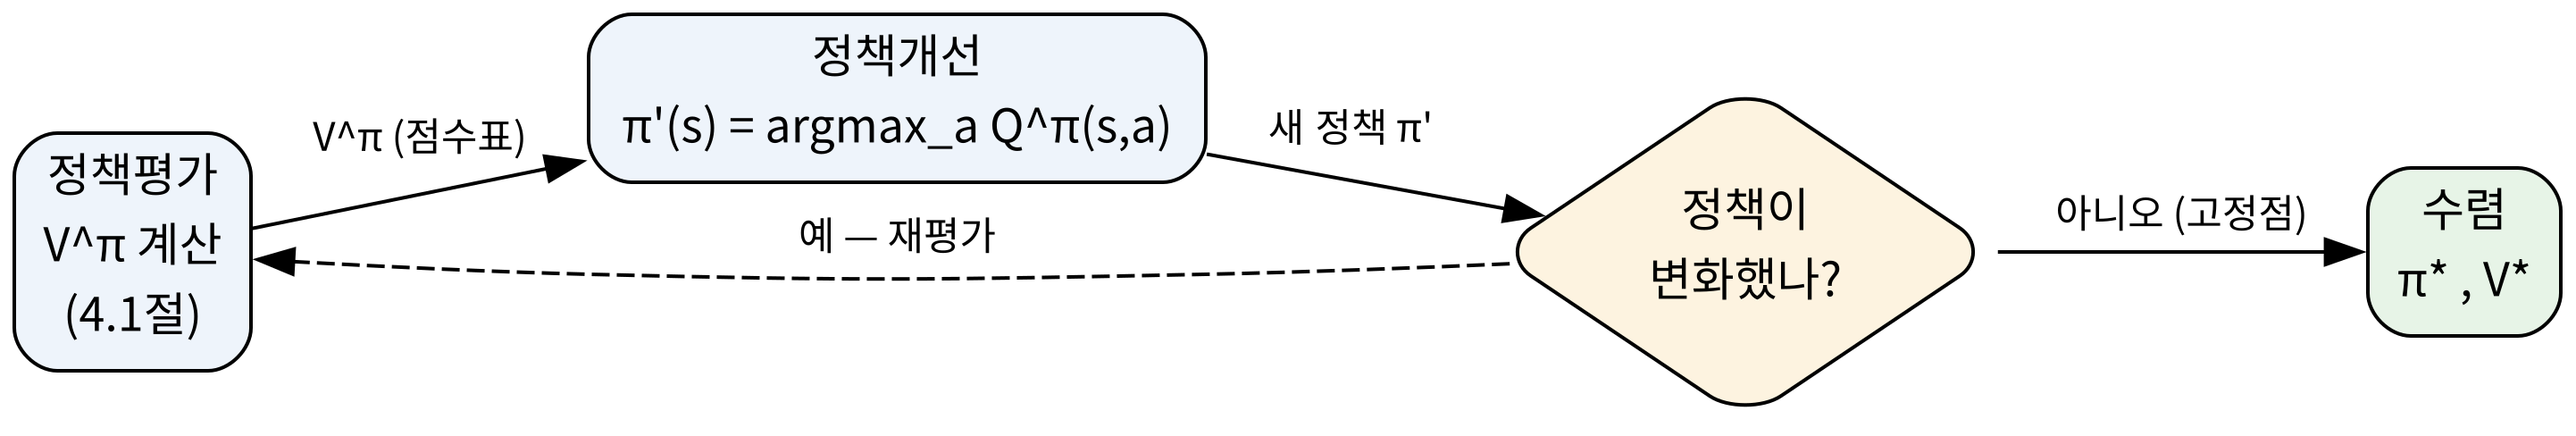
\includegraphics[width=0.5\linewidth]{ch04_2_policy_iteration_loop.png}
  \end{center}
  {\footnotesize 평가가 개선행동(각 행 argmax)을 산출하고, 개선이
  다음 평가의 대상(새 정책)을 산출. 두 단계가 \textbf{서로의
  출력을 입력}으로 먹는 구조.}
\end{frame}

\begin{frame}{왜 이 두 단계인가 + 개선 = $Q^\pi$ 표 행별 argmax}
  \begin{columns}[T]
    \begin{column}{0.5\textwidth}
      \kb{평가 alone}은 ``지금 정책이 \textbf{얼마나 좋은가}''
      만 답하고, ``어떻게 \textbf{고쳐야} 하는가''를 말해주지
      않음(4.1절 FAQ: 정책평가만으론 ``최적인가'' \textbf{판별
      불가}).
    \end{column}
    \begin{column}{0.5\textwidth}
      \kb{개선 alone}은 ``더 나은 행동''을 $V^\pi$ 기준으로
      판단해야 하는데, \textbf{정책이 바뀌면 $V^\pi$ 자체가
      바뀌어} 다시 계산 필요 $\to$ 한 발도 못 뺌.
    \end{column}
  \end{columns}
  \vskip0.6em
  \begin{block}{핵심 연결}
    개선 식의 우변 $R(s,a) + \gamma \sum_{s'} P(s'|s,a)\,
    V^\pi(s')$ 는 4.1절 \textbf{$Q^\pi(s,a)$ 그 자체}. 즉 4.1절이
    직접 채운 \kb{$Q^\pi$ 표가 정책개선의 점수표}이고, 개선은
    \textbf{각 행에서 최댓값을 따는 동작}. ``오른쪽'' 정책은
    자기 $Q^\pi$ 기준으로 \textbf{이미 바꿀 것이 없는} 상태
    (정책개선의 \kb{고정점}).
  \end{block}
\end{frame}

\begin{frame}{이론 (1/3): 질문 1 --- ``안 나빠지는가''?}
  \kq{질문 1. 개선한 정책이 정말로 안 나빠지는가?}
  (가치가 감소하면 ``최적해''라는 말 자체가 성립하지 않음.)
  \vskip0.5em
  \begin{block}{정책개선 정리 (단조 증가)}
    $\pi'$ 가 $\pi$ 를 \textbf{모든 상태에서 동시에} 개선한
    정책이면, 모든 $s$ 에서 $V^{\pi'}(s) \ge V^\pi(s)$.
  \end{block}
  \vskip0.4em
  \textbf{(i)} $V^{\pi'}$ 의 \textbf{정의}로, $\max$ 가 특정 성원
  이상이라는 자명한 사실:
  \[
  V^{\pi'}(s) = \max_a \left[R(s,a) + \gamma \sum_{s'}
  P(s'|s,a)\, V^{\pi'}(s')\right]
  \ge R(s,\pi'(s)) + \gamma \sum_{s'} P(s'|s,\pi'(s))\,
  V^{\pi'}(s')
  \]
\end{frame}

\begin{frame}{이론 (2/3): 증명은 두 줄}
  \textbf{(ii)} $\pi'(s)$ 의 \textbf{정의}($V^\pi$ 기준 argmax)로,
  $\pi'(s)$ 의 점수가 \textbf{모든} 행동 중 최대 $\to$ 현재
  $\pi(s)$ 보다 작을 수 없다:
  \[
  R(s,\pi'(s)) + \gamma \sum_{s'} P(s'|s,\pi'(s))\, V^\pi(s')
  \ge R(s,\pi(s)) + \gamma \sum_{s'} P(s'|s,\pi(s))\, V^\pi(s')
  = V^\pi(s)
  \]
  (마지막 등호: 벨만 기대방정식.)
  \vskip0.4em
  \textbf{두 줄 합치기:}
  \[
  V^{\pi'}(s) \;\ge\; R(s,\pi'(s)) + \gamma \sum_{s'}
  P(s'|s,\pi'(s))\, V^\pi(s') \;\ge\; V^\pi(s) \qquad \square
  \]
  \vskip0.4em
  \textbf{한 칸 손계산으로 체감.} ``왼쪽'' 정책($V = -10$ 모든
  칸)에서 \textbf{칸 3}: $Q(3, \text{left}) = -1 + 0.9 \times
  (-10) = -10$, $Q(3, \text{right}) = -1 + 0.9 \times 0 = -1$
  $\to$ right 이김 $\to$ $V^{\pi'}(3) = -1$ (목표에 1걸음),
  이전 $-10$ 보다 \textbf{나아짐}. 칸 0은 $\pi'$ 에서도
  왼쪽 $\to$ $V^{\pi'}(0) = -10$ \textbf{그대로} --- ``같거나
  낫다''는 \textbf{칸마다}(점순) 성립.
\end{frame}

\begin{frame}{이론 (3/3): 멈춤 = 최적, 그리고 유한성}
  \kq{질문 2. 멈춤 지점이 ``최적''인가?}
  멈춤 조건: \textbf{모든 $s$ 에서 $\pi(s) \in \arg\max_a
  Q^\pi(s,a)$} (자기 기준으로도 바꿀 것이 없음). 이 조건에서
  \textbf{직접} 읽히는 것:
  \[
  V^\pi(s) = \max_a \left[R(s,a) + \gamma \sum_{s'} P(s'|s,a)\,
  V^\pi(s')\right] \quad (\text{모든 } s)
  \]
  이것은 4.1절 \kb{벨만 최적방정식}. 해는 \textbf{유일}(4.3절
  바나흐)이므로 $V^\pi = V^{*}$ --- \kq{``개선의 고정점에서
  멈췄다'' = ``가치가 $V^{*}$ 다''}. (실습 `stable` 플래그의
  수학적 정체.)
  \vskip0.4em
  \begin{block}{유한성}
    결정론적 정책 총수 $m^n$(유한) + 가치 감소하지 않음(위
    정리) + \textbf{동점 처리 고정}(항상 최소 행동 번호) $\to$
    정책 수열은 유한집합 위 \textbf{결정적 함수의 궤적} $\to$
    언젠가 멈추거나 \textbf{주기 궤도} 진입. 주기 궤도 안의
    모든 정책은 \textbf{같은 가치}를 갖고, 그 값은 벨만
    최적방정식을 만족 $\to$ \textbf{어느 경우든 가치 기준의
    최적}. (고전적 결과: 바깥 반복 $\le n(m{-}1)$ 회.)
  \end{block}
\end{frame}

\begin{frame}{실전적 상한 + ``평가만 하면 안 된다''는 반례}
  단조 증가는 ``나빠지지 않는다''지만 ``얼마나 빨리 좋아지는가''
  는 주지 않음. 수축 성질(4.3절)로부터:
  \[
  \max_s \big|V^{\pi'}(s) - V^\pi(s)\big|
  \le \frac{1 - \gamma}{\gamma}\, \max_s \big|V^{*}(s) -
  V^\pi(s)\big|
  \]
  \begin{block}{실무적 메시지}
    \textbf{초기 정책이 아무리 엉망이어도, $\gamma$ 가 1에서
    충분히 멀지만 한 한 바퀴(평가+개선)에 오차가 \textbf{고정
    비율}($\gamma$ 배)로 줄어든다.} $\gamma = 0.99$ 처럼 1에
    가까우면 상한도 느려져 전체 비용이 크게 불어남.
  \end{block}
  \vskip0.4em
  \begin{block}{``평가만 하면 안 된다''는 반례}
    ``왼쪽'' 정책($V = -10$)을 \textbf{평가만} 하면 ``가치
    $-10$ 이다''가 \textbf{전부}. 개선 단계를 \textbf{한 번만}
    끼워도 \textbf{칸 3이 right로} 바뀌고($V(3): -10 \to -1$),
    그 정보가 다음 평가에서 \textbf{칸 2로, 다음에 칸 1로}
    퍼짐. \textbf{평가 alone}은 점수만 찍고, \textbf{개선
    단계}가 점수표를 ``갈아탈 방향''으로 번역 --- 두 단계의
    \textbf{곱}(점수 측정 × 방향 추출)이 정책 반복의 힘.
  \end{block}
\end{frame}

\begin{frame}[fragile]{실습: 5칸 GridWorld의 \texttt{policy\_iteration}}
\begin{lstlisting}
def policy_iteration(P, R, n_actions, gamma):
    policy = [1] * n_states   # 처음엔 무조건 오른쪽
    while True:
        V = policy_evaluation(P, R, policy, gamma)   # 1. 평가
        stable = True
        for s in range(n_states):                    # 2. 개선
            best_a = max(range(n_actions),
                         key=lambda a: R[s][a]
                             + gamma * sum(p*V[ns] for p, ns in P[s][a]))
            if best_a != policy[s]:
                policy[s] = best_a
                stable = False
        if stable:                    # 멈춤: 바뀐 것이 없으면
            return V, policy
\end{lstlisting}
  \vskip0.3em
  \textbf{실행 결과}: $V = [-3.439, -2.710, -1.900, -1.000,
  0.000]$, policy $= [1, 1, 1, 1, 0]$, \textbf{outer 2회},
  sweep 총합 \textbf{10}. 시작 정책이 이미 ``무조건 오른쪽''이라
  \textbf{첫 정책평가에서 곧바로 최적}이 나왔고, 개선 단계에서
  ``더 바꿀 게 없다''는 것만 한 번 확인. $V(0) = -3.439$ 는
  ``칸 0$\to$4까지 4번 이동의 할인 비용''
  $(-1 - 0.9 - 0.81 - 0.729 \approx -3.439)$ 과 정확히 일치.
\end{frame}

\begin{frame}{5칸 GridWorld의 $V^{*}$ 와 $\pi^{*}$ --- 정답 기준}
  \begin{columns}[T]
    \begin{column}{0.55\textwidth}
      \centering
      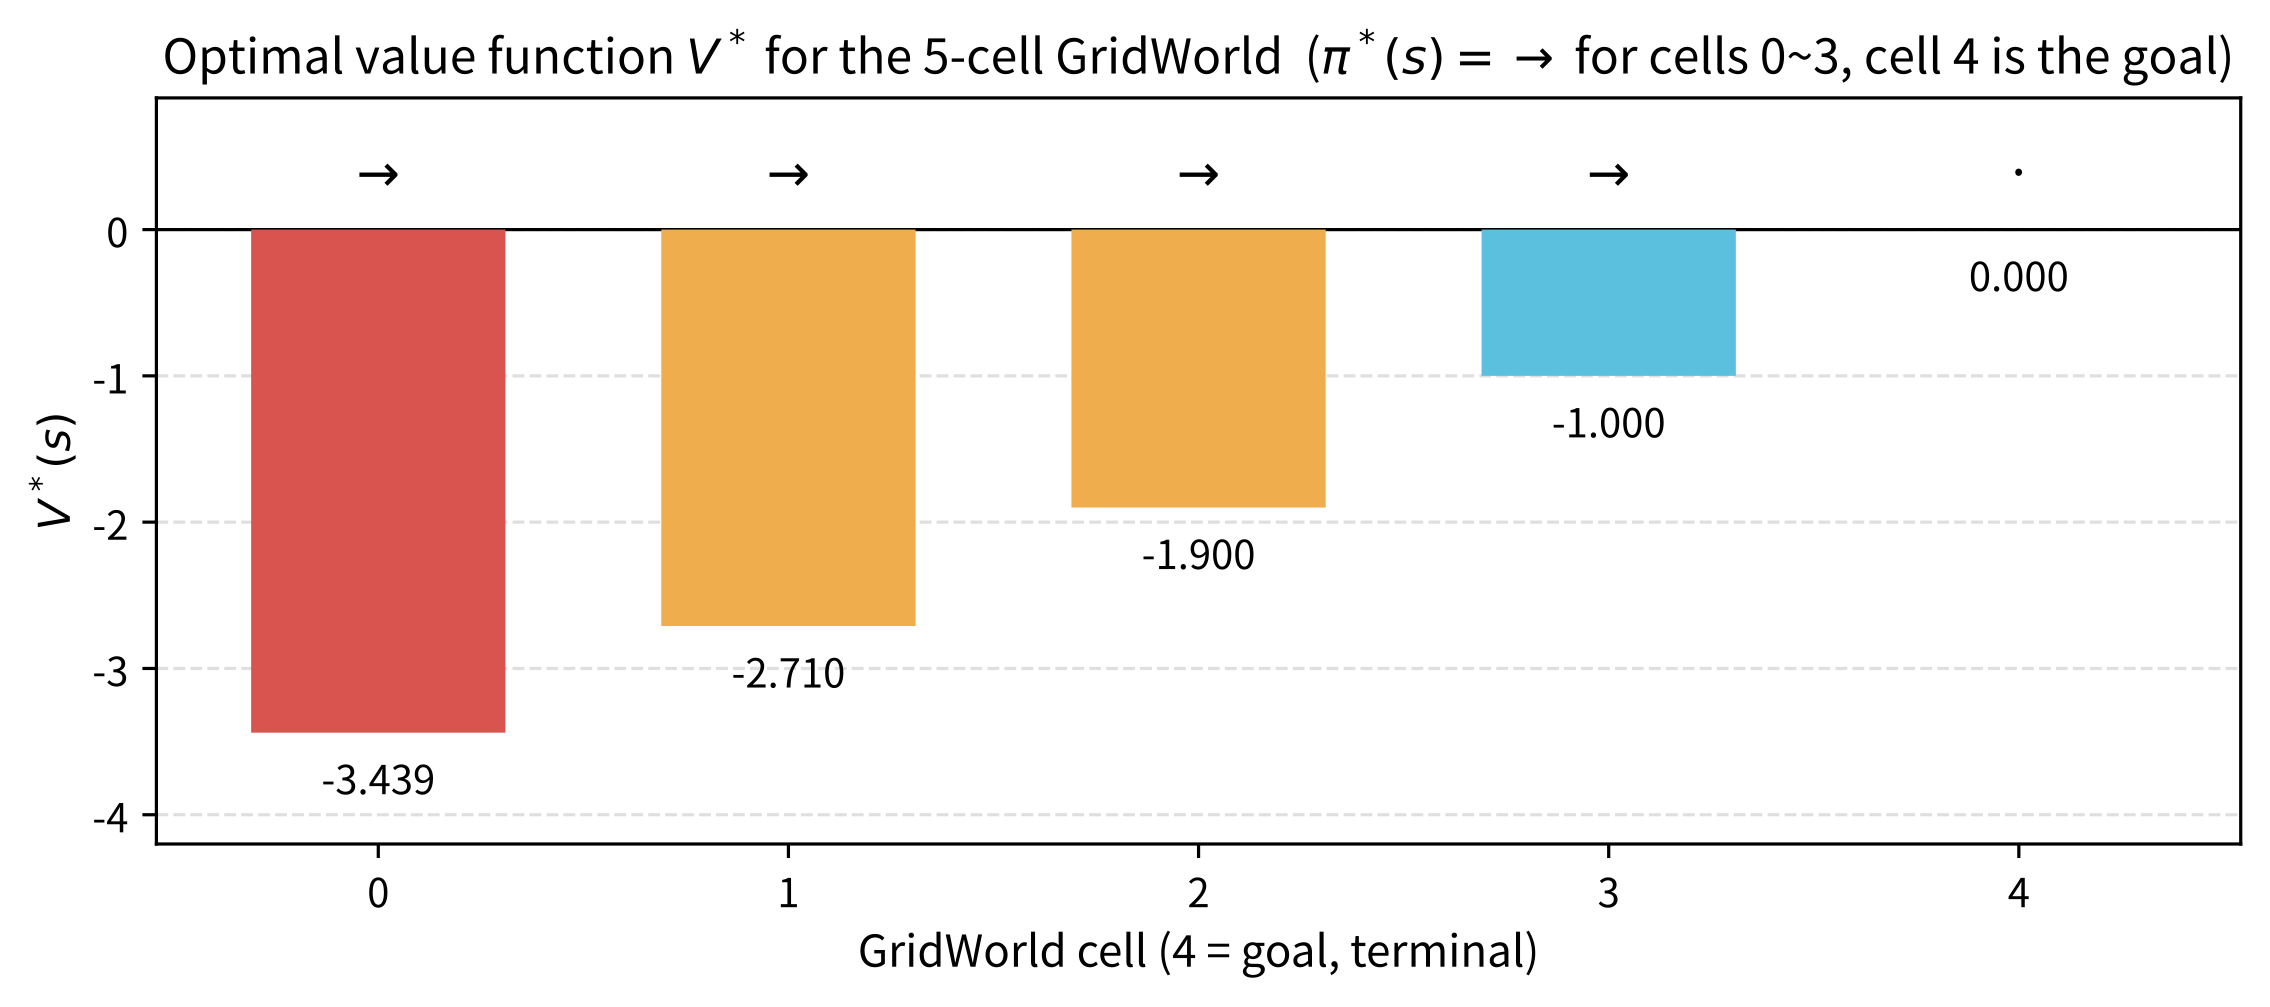
\includegraphics[width=\linewidth]{ch04_2_policy_iteration_walkthrough.png}
      \vskip0.3em
      {\footnotesize 5칸 GridWorld의 최적 가치함수 $V^{*}$ 와
      최적 정책 $\pi^{*}$.}
    \end{column}
    \begin{column}{0.43\textwidth}
      \begin{itemize}
        \item 칸 4(목표, 종료)에서 칸 0까지 각 칸의 $V^{*}$ 는
          ``\textbf{목표까지 걸음 수의 할인 비용}'': $-1$,
          $-1 - 0.9$, $-1 - 0.9 - 0.81$, $\ldots$
        \item 최적 정책: \textbf{모든 칸에서 ``오른쪽''}.
        \item 이 $V^{*} = [-3.439, -2.710, -1.900, -1.000, 0]$ 가
          \textbf{이번 장 모든 알고리즘}(정책 반복·수정된
          정책 반복·가치 반복)의 \textbf{정답 기준}.
      \end{itemize}
    \end{column}
  \end{columns}
  \vskip0.5em
  {\footnotesize 정책 반복 수렴 속도는 \textbf{초기 정책을 얼마나
  잘 골랐는지에 따라 크게} 달라짐 --- 이제 의도적으로 ``최악의
  출발''을 해본다.}
\end{frame}

\begin{frame}{최악의 출발: ``왼쪽''에서 시작하면 한 칸씩 전파}
  ``왼쪽'' 정책(벽에 붙어 무한 루프 $\to$ $V = -10$)에서 시작:
  \small
  \begin{tabular}{@{}llrl@{}}
    \toprule
    outer & 정책 & sweep & $V$ \\
    \midrule
    1 & $[L, L, L, L, \cdot] \to [L, L, L, R, \cdot]$ & 133 & $[-10, -10, -10, -10, 0]$ \\
    2 & $[L, L, L, R, \cdot] \to [L, L, R, R, \cdot]$ & 133 & $[-10, -10, -10, -1, 0]$ \\
    3 & $[L, L, R, R, \cdot] \to [L, R, R, R, \cdot]$ & 133 & $[-10, -10, -1.9, -1, 0]$ \\
    4 & $[L, R, R, R, \cdot] \to [R, R, R, R, \cdot]$ & 133 & $[-10, -2.71, -1.9, -1, 0]$ \\
    5 & $[R, R, R, R, \cdot] \to$ (변화 없음) & 5 & $[-3.44, -2.71, -1.9, -1, 0]$ \\
    \bottomrule
  \end{tabular}
  ($L$ = left, $R$ = right, $\cdot$ = 목표. \textbf{총
  $133 \times 4 + 5 = 537$ sweep}.)
  \vskip0.5em
  \begin{block}{왜 \textbf{칸 3}이 가장 먼저 바뀌는가?}
    outer 1에서 $V^{\text{left}}$ 가 모두 $-10$ 인 상태에서
    $Q(3, \text{left}) = -10$ 인데 $Q(3, \text{right}) = -1 +
    0.9 \times 0 = -1$ --- \textbf{목표($V = 0$)가 바로 옆}인
    칸 3에서만 right가 압도적으로 낫다. 칸 0$\sim$2는 $Q(s,
    \text{right}) = -10$ 으로 left와 \textbf{동점} $\to$ `max`가
    기존 left를 \textbf{그대로 둔다}.
  \end{block}
\end{frame}

\begin{frame}{정보 전파(바깥 반복 버전) + 세 방법 나란히}
  \begin{itemize}
    \item outer 2에서 칸 3의 가치가 $-1$ 로 갱신되자 \textbf{칸
      2}에서 right가 이긴다: $Q(2, \text{right}) = -1 + 0.9
      \times (-1) = -1.9 > -10$. 이 ``\textbf{목표가 가까워졌다}''
      는 정보가 바깥 반복마다 \textbf{한 칸씩 왼쪽으로 전파} ---
      4.1절 ``한 sweep에 한 칸 전파''의 \textbf{바깥 반복 버전}.
  \end{itemize}
  \vskip0.4em
  \begin{block}{같은 알고리즘, 시작 정책만 바꿔도}
    ``오른쪽'' 출발: 총 sweep \textbf{10} $\;$vs$\;$ ``왼쪽''
    출발: 총 sweep \textbf{537} --- \textbf{약 54배} 차이.
    ``정책 반복 속도는 초기 정책에 \textbf{민감하다}''의 실질,
    그리고 4.3절 가치 반복이 ``초기 정책에 \textbf{무관하게}
    $V^{*}$ 로 직접 간다''는 설계 의도의 동기.
  \end{block}
  \vskip0.4em
  {\small ``왼쪽'' 출발, $\theta = 10^{-6}$ 기준 세 방법:
  \begin{tabular}{@{}lccc@{}}
    \toprule
    방법 & 바깥 반복 & 내부 sweep & \textbf{총 sweep} \\
    \midrule
    정책 반복 (완전 수렴) & 5 & $133 \times 4 + 5$ & \textbf{537} \\
    수정된 정책 반복 ($k = 2$) & 5 & $2 \times 5$ & \textbf{10} \\
    수정된 정책 반복 ($k = 1$) = 가치 반복 & 5 & $1 \times 5$ & \textbf{5} \\
    \bottomrule
  \end{tabular}}
  {\footnotesize \textbf{과대해석 금지} --- 위는 벽에 붙은 무한
  루프를 $\gamma = 0.9$ 로 할인까지 다 풀어내는 \textbf{최악
  경로}. 다른 MDP에선 한 번에 여러 칸 바뀌어 완전 수렴이 더
  싸질 수도. 표에서 \textbf{확실한 것만}: \textbf{세 방법은
  모두 정확히 같은 $V^{*}$ 와 같은 최적에 도달}.}
\end{frame}

\begin{frame}[fragile]{수정된 정책 반복: $k$ sweep만 평가 후 개선}
  \textbf{정책평가를 끝까지 수렴시키지 않고 $k$ sweep만} 돌린
  뒤 \textbf{바로 개선}(modified policy iteration):
\begin{lstlisting}
def modified_policy_iteration(P, R, n_actions, gamma, k):
    """k = 내부 정책평가 sweep 수. k=1이면 가치 반복과 동일."""
    policy = [0] * n_states   # "왼쪽"에서 시작
    V = [0.0] * n_states
    while True:
        for _ in range(k):                   # 평가: k sweep만
            for s in range(n_states):
                a = policy[s]
                V[s] = R[s][a] + gamma * sum(p * V[ns] for p, ns in P[s][a])
        stable = True
        for s in range(n_states):            # 개선: argmax
            best_a = max(range(n_actions),
                         key=lambda a: R[s][a] + gamma * sum(p * V[ns] for p, ns in P[s][a]))
            if best_a != policy[s]:
                policy[s] = best_a
                stable = False
        if stable:
            return V, policy
\end{lstlisting}
  \vskip0.2em
  실행(모두 ``왼쪽'' 출발, 정책 변화 여부로 멈춤): $k = 1, 2, 3,
  5$ 모두 \textbf{바깥 반복 5}, 최종 $V = [-3.439, -2.710,
  -1.900, -1.000, 0]$ \textbf{동일} (총 sweep = $5k$).
\end{frame}

\begin{frame}{$k = 1$ 은 가치 반복: ``같은 연산의 다른 분해''}
  \begin{block}{$k = 1$ 확인}
    ``평가 1 sweep'' = 각 상태의 $V$ 를 $\max_a$[보상 + 할인
    미래값]으로 갱신하는 한 바퀴(정책을 ``평가 중''에 argmax로
    교체), ``개선''은 이미 그 sweep 안의 argmax로 \textbf{흡수}.
    두 표현(평가+개선 분리 vs 한 sweep에 통합)은 \textbf{동일한
    연산의 다른 분해}.
  \end{block}
  \vskip0.4em
  $k$ 를 1에서 $\infty$(완전 수렴)로 늘리면 가치 반복에서 정책
  반복으로 \textbf{연속적으로} 이어진다:
  \[
  \text{가치 반복}(k = 1) \to k = 2 \to k = 3 \to \cdots
  \to \text{정책 반복}(k = \infty)
  \]
  \vskip0.4em
  \begin{block}{$k$ 가 작아도 왜 최적인가}
    $k$ sweep의 정책평가 연산 $T^{\pi, k}$ 는 ``$T^\pi$ 를 $k$ 번
    적용''이므로 여전히 \textbf{$\gamma^k$-축소 사상}. 바나흐
    정리(4.3절)와 ``고정점에서 멈추면 최적'' 논증은 \textbf{변함
    없이 적용} --- \textbf{수렴 속도만} $k$ 에 따라 변한다.
  \end{block}
  {\footnotesize 실무적으로 $k$ 는 ``평가 한 sweep의 비용 대비
  얼마나 정확한 $V^\pi$ 가 필요한가''의 \textbf{trade-off}.}
\end{frame}

\begin{frame}{자주 하는 실수}
  \begin{itemize}
    \item \kb{``평가 $\to$ 개선'' 순서를 뒤집거나, 개선 전에
      평가를 안 한다.} 개선 식의 $V^\pi$ 는 \textbf{현재} 정책
      가치. \textbf{이전} $V$ 로 개선하면 ``낡은 점수표로
      갈아탈 방향을 고르는'' 셈 $\to$ 단조 증가 전제가 \textbf{깨짐}.
      \texttt{V = policy\_evaluation(...)}을 \texttt{while}
      \textbf{안쪽}에 두는 것이 맞고, 루프 밖에서 한 번만 계산해
      재사용하면 안 된다.
    \item \kb{개선 단계에서 일부 상태만 고친다.} (예: ``값이
      가장 나쁜'' 상태부터) 단조 증가는 \textbf{모든 상태를
      동시에} 개선할 때 성립. 순서대로 하나씩 고치면 ``고친
      상태의 기준 $V$ 와 안 고친 상태의 기준 $V$ 가 \textbf{다를}''
      수 있어 증명이 직접 적용되지 않음(변형도 보통 수렴하지만
      \textbf{다른 논증} 필요).
    \item \kb{$\arg\max$ 동점을 ``임의로'' 처리하고 결과를 믿는다.}
      동점 MDP에선 \textbf{결과 정책}이 처리 규칙(행동 순서,
      `max` 첫 발견)에 따라 \textbf{달라지지만} \textbf{가치
      ($V^{*}$)는 항상 같음}. ``유일한 최적''이 아니라
      ``\textbf{최적 중 하나}''. `max`가 첫 최댓값을 반환해
      행동 순서 $[0,1,2,\ldots]$ 에 \textbf{편향}.
    \item \kb{``몇 번이면 끝나는지'' 문제 없이 예측한다.}
      $n(m{-}1)$ 은 \textbf{최악의 경우} 상한. 실제로는 초기
      정책에 따라 2번$\sim$상한에 가까움까지 다양. ``예상 소요
      시간''으로 착각하면 큰 MDP에서 당황.
  \end{itemize}
  {\footnotesize 다섯 번째: \texttt{delta < theta}(내부 평가
  수렴)와 \texttt{stable}(외부 ``변화 여부'')는 \textbf{서로
  다른 판정 두 개}. $\theta$ 를 너무 느슨하게(예: 1) 쓰면
  ``거의 안 된'' $V^\pi$ 로 개선 $\to$ 잘못된 argmax.}
\end{frame}

\begin{frame}[fragile]{실습: 동점 MDP --- 정책은 다르고, $V^{*}$ 는 유일}
  ``동점이 있으면 결과 정책은 달라져도 \textbf{가치는 항상
  같다}''를 작은 MDP로 확인. 상태 0이 \textbf{두 개의 문}(행동
  0, 1)을 갖고 각각 방 1 / 방 2(각각 $+1$ 주고 \textbf{self-loop
  종료})로 가는 3상태 MDP:
\begin{lstlisting}
# 상태 0: 두 개의 문. 방 1,2: self-loop (종료)
P[0][0], R[0][0] = [(1.0, 1)], 1.0    # 문 a0 -> 방 1 (+1, 종료)
P[0][1], R[0][1] = [(1.0, 2)], 1.0    # 문 a1 -> 방 2 (+1, 종료)
P[1][0], R[1][0] = [(1.0, 1)], 0.0    # 방 1: self-loop
P[2][1], R[2][1] = [(1.0, 2)], 0.0    # 방 2: self-loop
# (나머지 P, R은 0. 방 1·2는 어떤 행동을 해도 자기 자신)

def policy_iteration_tie(P, R, n_actions, gamma, tie_break):
    policy = [0] * n_states
    while True:
        V = policy_evaluation(P, R, policy, gamma)
        stable = True
        for s in range(n_states):
            qs = [R[s][a] + gamma * sum(p*V[ns] for p, ns in P[s][a])
                  for a in range(n_actions)]
            best = max(qs)
            cands = [a for a in range(n_actions) if abs(qs[a] - best) < 1e-12]
            chosen = cands[0] if tie_break == 'first' else cands[-1]
            if chosen != policy[s]:
                policy[s] = chosen
                stable = False
        if stable:
            return V, policy
\end{lstlisting}
\end{frame}

\begin{frame}{동점 실행 결과: 정책 2가지, $V^{*}$ 1가지}
  \small
  \begin{tabular}{@{}lll@{}}
    \toprule
    동점 처리 & 결과 policy & $V$ \\
    \midrule
    \texttt{'first'} (최소 행동 번호) & $[0, 0, 0]$ & $[1.0000, 0.0000, 0.0000]$ \\
    \texttt{'last'} (최대 행동 번호) & $[1, 1, 1]$ & $[1.0000, 0.0000, 0.0000]$ \\
    \bottomrule
  \end{tabular}
  \vskip0.8em
  \begin{itemize}
    \item 상태 0에서 두 행동: $Q(0, \text{left}) = 1 + 0 = 1$,
      $Q(0, \text{right}) = 1 + 0 = 1$ --- \textbf{완벽한 동점}.
    \item \textbf{결과 정책은 완전히} 다르고($[0,0,0]$ vs
      $[1,1,1]$), $V$ 는 \textbf{완전히} 같다($[1, 0, 0]$).
  \end{itemize}
  \vskip0.6em
  \begin{block}{유한성 논증이 약속한 그대로}
    동점 MDP에서 \textbf{``최적 정책''은 유일하지 않을 수
    있다}(여기서 2개 이상 공존), 하지만 \textbf{``최적 가치
    $V^{*}$''는 유일}. 실전에서 동점이 중요한 이유: (a) 같은
    $V^{*}$ 를 전제로 정책은 \textbf{추가 기준}(더 안전한 행동
    선호, 물리적 비용)으로 골라야 하며, (b) ``정책이 다르다''는
    이유로 ``알고리즘 실패''로 판단하면 \textbf{안 된다} ---
    \textbf{$V^{*}$ 가 일치하면 성공}.
  \end{block}
\end{frame}

\begin{frame}{FAQ}
  \begin{itemize}
    \item \textbf{Q. 정책개선에서 ``더 나은 행동''이 여러 개
      동점이면?} 이론적으로 동점 중 \textbf{아무거나} 골라도
      성질(가치 감소 안 함) 유지. 실전: `max`가 \textbf{첫
      번째} 최댓값 반환 $\to$ 순서에 따라 결과 \textbf{정책}은
      달라져도 \textbf{가치($V$)는 항상 같음}.
    \item \textbf{Q. 정책평가를 항상 끝까지(수렴까지) 해야
      하나요?} \textbf{아니다} --- 수렴시키지 않고 몇 번만
      돌린 뒤 바로 개선해도 결국 \textbf{최적 정책으로 수렴}
      (수정된 정책 반복). 극단적으로 \textbf{딱 한 번}만 하면
      $\to$ 4.3절 \textbf{가치 반복과 정확히 같아짐}.
    \item \textbf{Q. ``왼쪽'' 537 vs ``오른쪽'' 10 sweep,
      같은 알고리즘인데 왜?} \textbf{평가 단계의 sweep 수}가
      초기 정책에 따라 달라짐. ``왼쪽''은 벽에 붙은 무한 루프를
      $10^{-6}$ 까지 풀어내야 133 sweep, ``오른쪽''은 5 sweep.
      바깥 반복 \textbf{횟수}도 5 vs 2. 두 요인이 \textbf{곱해져}
      총 계산량이 초기 정책에 민감.
    \item \textbf{Q. 실전에서 어디에 쓰나요?} 상태 공간이
      \textbf{작고} $P, R$ 를 \textbf{정확히 아는} 문제(작은
      그리드, 재고 관리, 스케줄링)엔 지금도 그대로. ``$P$ 를
      모른다''(Ch.\,5--7)나 ``상태가 너무 크다''(Ch.\,9 DQN,
      Mnih et al., 2015)엔 직접 쓰지 \textbf{않고}, 대신 이 절의
      \textbf{논증 구조}(평가$\to$개선$\to$단조 증가$\to$
      고정점$=$최적)가 TD·Q-learning의 ``왜 수렴하는가''
      논의의 \textbf{뼈대}로 재사용. (DQN의 \textbf{residual
      검사} = ``Q-망이 벨만 최적방정식을 만족하는가''.)
  \end{itemize}
\end{frame}

\begin{frame}{4.2절 마무리}
  \begin{block}{4.2절에서 만든 것}
    \begin{enumerate}
      \item \kb{정책 반복} = 평가 $\to$ 개선을 번갈아, ``개선이
        아무것도 안 바꿀 때'' 멈춤.
      \item \kb{정책개선 정리(단조 증가)} + \kb{유한성}
        $\to$ ``멈추면 최적''(멈춤 = 벨만 최적방정식 성립,
        해 유일 $\Rightarrow$ $V^\pi = V^{*}$).
      \item \kb{수정된 정책 반복}(평가 $k$ sweep + 개선) ---
        $k = 1$ 은 \textbf{가치 반복}, $k = \infty$ 는
        \textbf{정책 반복}. ``같은 알고리즘의 $k$ 스펙트럼''.
    \end{enumerate}
  \end{block}
  \vskip0.5em
  {\footnotesize 예습 확인 문제: ① ``멈춤 = 벨만 최적방정식
  성립'' 논증을 세 문장 이내로 요약. ② outer 3에서 $V(2) =
  -1.9 = -1 + 0.9 \times V(3) = -1 - 0.9$ (``칸 2에서 목표까지
  2걸음의 할인 비용'') 검증. ③ $k = 10$ 인
  \texttt{modified\_policy\_iteration}의 총 sweep = $5 \times 10
  = 50$, 바깥 반복 \textbf{5}($k$ 와 무관). ④ $\gamma = 0.99$,
  $\Delta_0 = 13.44$ 에서 $\Delta < 0.01$ 까지 $13.44 \times
  0.99^k < 0.01$ 을 $\log$ 로 풀면 $k \approx 717$ 바퀴
  $\Rightarrow$ 정책 반복도 $\gamma$ 에 민감.}
\end{frame}

\section{4.3 가치 반복, 수렴 증명, 그리고 모델 기반이라는 전제}

\begin{frame}[fragile]{가치 반복: ``한 줄 차이''가 최적을 찾는다}
  \kb{가치 반복} (Value Iteration)은 정책평가와 개선을 합쳐서,
  \textbf{평가를 끝까지 수렴시키지 않고 딱 한 번만} 하고
  \textbf{바로 개선}하는 것을 매 스텝 반복 --- \textbf{벨만
  최적방정식 자체를 반복 대입으로 직접 푸는 것}:
\begin{lstlisting}
def value_iteration(P, R, n_actions, gamma, theta=1e-6):
    n_states = len(P)
    V = [0.0] * n_states
    while True:
        delta = 0
        for s in range(n_states):
            v_new = max(R[s][a] + gamma * sum(prob * V[next_s]
                        for prob, next_s in P[s][a])
                        for a in range(n_actions))   # <- max_a
            delta = max(delta, abs(v_new - V[s]))
            V[s] = v_new
        if delta < theta:
            break
    policy = [max(range(n_actions),
                  key=lambda a: R[s][a] + gamma * sum(prob * V[next_s]
                              for prob, next_s in P[s][a]))
              for s in range(n_states)]
    return V, policy
\end{lstlisting}
  \vskip0.2em
  {\footnotesize 4.1절 \texttt{policy\_evaluation}과 \textbf{딱
  한 줄이 달라}다.}
\end{frame}

\begin{frame}{``한 줄''의 차이: $a = \pi(s)$ $\to$ $\max_a$}
  \texttt{a = policy[s]}로 고른 한 행동이 아니라, \texttt{max\_a
  [\ldots]}로 \textbf{각 상태에서 가장 좋은 행동}을 \textbf{그때그때
  고르는 것}이 전부다. 이 ``한 줄''이
  \kq{``주어진 정책을 평가''}와 \kq{``최적인 정책을 찾기''}를
  가르는 \textbf{전부}.
  \vskip0.5em
  4.1절 벨만 연산자 관점에서 더 명확하다:
  \begin{itemize}
    \item \kb{정책평가} = \textbf{정책 연산자} $T^\pi$ 를
      반복하는 것: $V \xrightarrow{T^\pi} \cdots$
    \item \kb{가치 반복} = \textbf{최적 연산자}
      $T^{*} V(s) = \max_a [R + \gamma \sum P\, V]$ 를 반복하는
      것: $V \xrightarrow{T^{*}} V_1 \xrightarrow{T^{*}} V_2 \to
      V^{*}$.
  \end{itemize}
  둘은 4.1절 벨만방정식 2$\times$2 표에서 \textbf{``기대''
  열}과 \textbf{``최적'' 열}의 차이에 해당.
\end{frame}

\begin{frame}{$T^\pi \to T^{*}$: 기대 열 vs 최적 열}
  벨만 연산자 관점에서: 정책평가 = \textbf{정책 연산자} $T^\pi$
  를 반복($V \xrightarrow{T^\pi} \cdots$), 가치 반복 =
  \textbf{최적 연산자} 를 반복:
  \[
  T^{*} V(s) = \max_a \left[R(s,a) + \gamma \sum_{s'} P(s'|s,a)\,
  V(s')\right]
  \qquad
  (V \xrightarrow{T^{*}} V_1 \xrightarrow{T^{*}} V_2 \to V^{*})
  \]
  4.1절 2$\times$2 표에서 \textbf{``기대'' 열 vs ``최적''
  열}의 차이에 해당.
  \vskip0.6em
  \begin{block}{$T^{*}$ 를 $k$ 번 적용 = ``$k$스텝만 내다보기''}
    5칸 GridWorld, $V_0 = [0,0,0,0,0]$ 로 시작해 $T^{*}$ 를
    \textbf{한 번씩만}(synchronous) 적용:
    \begin{tabular}{@{}rrrrr@{}}
      \toprule
      $k$ & $V_k(0)$ & $V_k(1)$ & $V_k(2)$ & $V_k(3)$ \\
      \midrule
      0 & 0.000 & 0.000 & 0.000 & 0.000 \\
      1 & $-1.000$ & $-1.000$ & $-1.000$ & $-1.000$ \\
      2 & $-1.900$ & $-1.900$ & $-1.900$ & $-1.000$ \\
      3 & $-2.710$ & $-2.710$ & $-1.900$ & $-1.000$ \\
      4 & $-3.439$ & $-2.710$ & $-1.900$ & $-1.000$ \\
      5 & $-3.439$ & $-2.710$ & $-1.900$ & $-1.000$ \\
      \bottomrule
    \end{tabular}
  \end{block}
\end{frame}

\begin{frame}{지평선이 한 칸씩 넓어지고, $k = 4$ 에서 고정}
  $V_k(s)$ 의 해석: ``$s$ 에서 출발해 \textbf{정확히 $k$스텝만}
  최적으로 행동(이후 보상 0)할 때의 할인 누적 보상''.
  \begin{itemize}
    \item $V_1$: ``한 걸음만'' --- 목표(칸 4) 아니면 전부 $-1$.
    \item $V_2$: 칸 0,1,2는 두 걸음 안에 못 닿아 $-1.9$, 칸 3은
      한 걸음이면 목표라 $-1$.
    \item $V_3$: 칸 0은 여전히 못 닿아 $-2.71$.
  \end{itemize}
  \vskip0.4em
  \begin{block}{지평선(horizon)이 매 스텝 한 칸씩 오른쪽으로 넓어진다}
    4.1절 ``정보는 한 sweep에 한 칸 전파''와 \textbf{정확히
    같은 현상}. $k = 4$ 가 되면 칸 0에서도 목표까지 거리(4칸)를
    다 보게 되어 \textbf{고정}($-3.439$). \textbf{$k = 4$ 에서
    더 이상 안 변한다} --- 목표까지 \textbf{최장 거리 4}이므로
    ``4스텝만''과 ``무한히'' 보는 것이 \textbf{같은 답}.
  \end{block}
  \vskip0.4em
  \begin{block}{이 직관의 두 의미}
    (1) \textbf{$k$ 가 충분히 크면 $V_k$ 가 $V^{*}$ 에 수렴} ---
    ``왜''가 아니라 \textbf{``몇 스텝이면''의 눈금자}(목표까지
    최대 거리 + $\gamma^k$ 가 충분히 작아질 때까지의 $k$).
    (2) ``내다보는 스텝 수를 늘려가며 근사''는 Ch.\,14 \kb{MPC}
    (Mayne et al., 2000)과 \textbf{동일 사상} --- MPC는 매
    결정 시점 ``앞으로 $k$스텝만''을 고르고 $k$ 키울수록 장기
    계획 반영, 가치 반복은 $k$ 를 \textbf{스스로 키워}
    $k = \infty$(= $V^{*}$)까지 닫아가는 절차.
  \end{block}
\end{frame}

\begin{frame}[fragile]{실습: 정책반복 vs 가치반복, 같은 고정점}
\begin{lstlisting}
V_vi, policy_vi = value_iteration(P, R, n_actions, gamma)
# V      = [-3.439, -2.710, -1.900, -1.000, 0.000]  # 정책반복과 동일
# policy = [1, 1, 1, 1, 0]                          # 정책반복과 동일
# 반복 횟수: 5
\end{lstlisting}
  \begin{columns}[T]
    \begin{column}{0.5\textwidth}
      \centering
      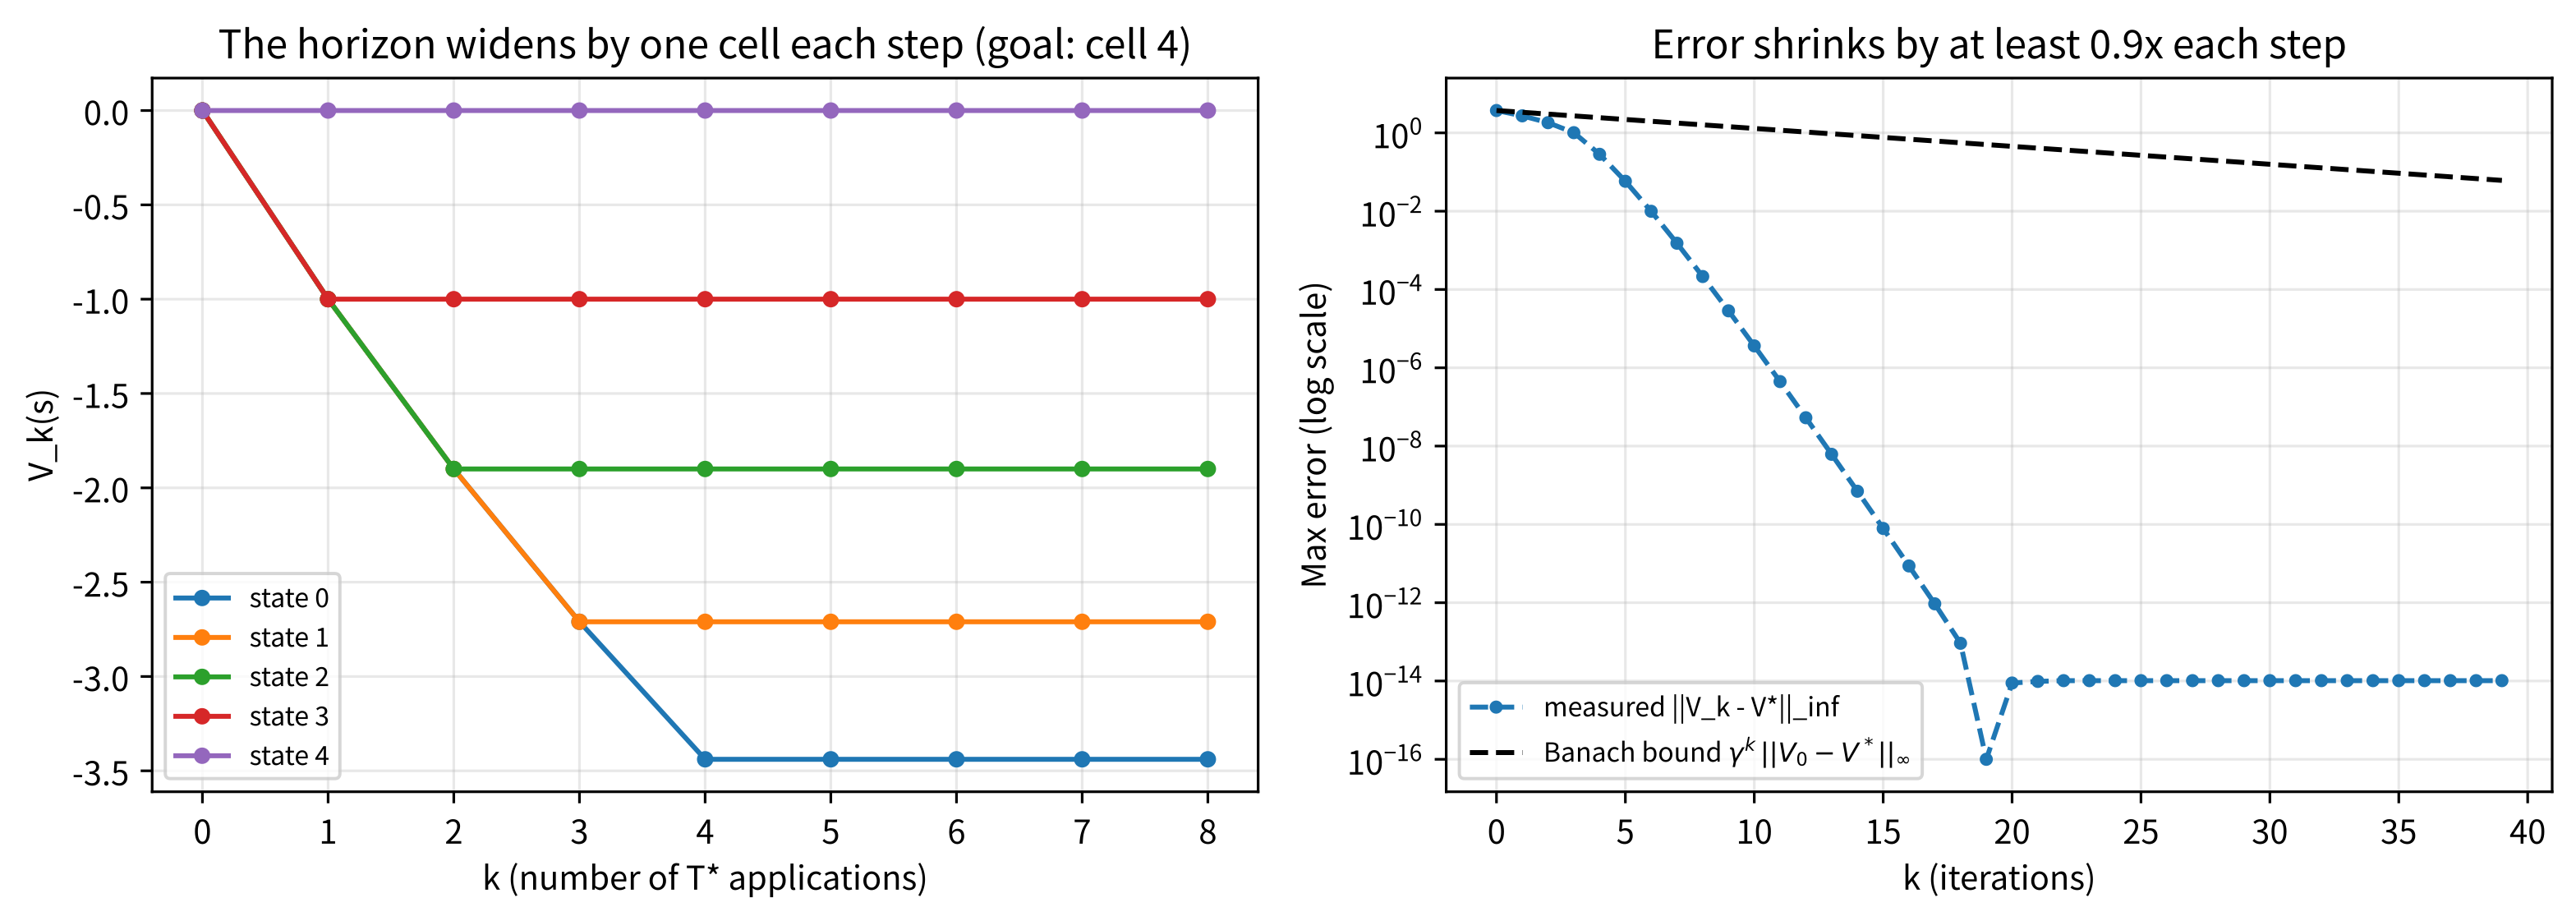
\includegraphics[width=\linewidth]{ch04_3_value_iteration_horizon.png}
      \vskip0.3em
      {\footnotesize (좌) 지평선을 한 칸씩 넓혀가는 과정,
      (우) 오차 로그 곡선 --- 실측 오차(파란 점선)가 바나흐
      상한 $\gamma^k$(검정) \textbf{아래}를 따라감.}
    \end{column}
    \begin{column}{0.48\textwidth}
      \begin{itemize}
        \item 두 알고리즘 모두 \textbf{정확히 같은} $V^{*}$ 와
          최적 정책 --- \textbf{같은 고정점}(벨만 최적방정식)
          을 찾아가기 때문(해 유일, 아래 증명).
        \item ``수렴까지 \textbf{계산의 성격}''이 다름:
          정책반복은 바깥 반복 2번(내부 평가 sweep 총 10) vs
          가치반복은 단일 루프 5번.
        \item \textbf{일반적으로}: 정책반복은 바깥 반복은 적지만
          각 반복(평가)이 \textbf{무거울 수} 있고, 가치반복은
          \textbf{가볍지만} 반복 횟수가 더 필요할 수 있음.
          어느 쪽이 총 계산량이 적은지는 \textbf{문제마다 다름}.
      \end{itemize}
    \end{column}
  \end{columns}
\end{frame}

\begin{frame}{in-place vs synchronous: 여기서 왜 일치하나?}
  위 \texttt{value\_iteration}은 \textbf{in-place}(sweep
  \textbf{중}에도 갱신된 값을 사용)인데, 이 5칸 예에서는
  synchronous와 \textbf{매 스텝 값이 정확히 일치} --- 위 표의
  $V_k$ 행이 바로 \textbf{두 버전 공통의 추적궤적}.
  \vskip0.4em
  \begin{block}{이유: 최적 전이가 오른쪽 방향뿐}
    이 GridWorld의 \textbf{최적 전이가 오른쪽 방향만}이므로,
    sweep을 \textbf{0$\to$4 순서}로 돌리면 갱신 정보가 ``아직 안
    갱신된 $\to$ 이미 갱신된 상태로만'' 흘러간다(sweep 순서가 정보
    흐름과 \textbf{반대} 방향).
  \end{block}
  \vskip0.4em
  \begin{block}{sweep 순서 = 정보 흐름 방향이면}
    sweep 순서가 정보 흐름과 \textbf{같은} 방향(예: 상태 순서를
    4$\to$0 으로 뒤집으면)이면 in-place가 \textbf{한 sweep 안에
    정보를 더 멀리 전파해 \textbf{더 빠르게} 수렴}할 수 있다
    (4.1절). \textbf{같은 고정점}으로 수렴한다는 보장은
    \textbf{변하지 않음} --- 차이는 \textbf{속도}뿐.
  \end{block}
\end{frame}

\begin{frame}{정책반복과 가치반복: ``같은 알고리즘의 두 극한''}
  수정된 정책 반복을 $k$ 에 따라 나열(5칸, 4.2절의 초기 정책
  ``무조건 오른쪽''에서 출발, $V$ 는 sweep마다 이어서 쓰는
  warm start):
  \begin{tabular}{@{}clccc@{}}
    \toprule
    $k$ & 이름 & 바깥 반복 & 총 sweep & 결과 $V(0)$ \\
    \midrule
    1 & \textbf{가치 반복} & 5 & 5 & $-3.439$ \\
    2 & 수정된 정책반복 & 4 & 8 & $-3.439$ \\
    4 & 수정된 정책반복 & 2 & 8 & $-3.439$ \\
    $\infty$ & \textbf{정책 반복} & 2 & 10 & $-3.439$ \\
    \bottomrule
  \end{tabular}
  \vskip0.6em
  \begin{block}{``다른 알고리즘''이 아니라 \textbf{연속 스펙트럼}}
    가치반복과 정책반복은 따로따로 배운 ``다른 알고리즘''이 아니라,
    \textbf{같은 프레임워크의 연속 스펙트럼 양 끝단}이다. $k$ 를
    키우면 \textbf{바깥 반복은 줄고} 각 반복이 \textbf{무거워지며},
    극단 $k = 1$ 이 \textbf{가치반복}, $k = \infty$ 가 \textbf{정책
    반복}.
  \end{block}
\end{frame}

\begin{frame}{$k$ 가 적어도 최종 답은 그대로}
  \kq{``평가 횟수 $k$ 가 적다고 최종 답이 안 나온다?''}
  \vskip0.5em
  \begin{itemize}
    \item $k = 1$ 부터 $k = \infty$ 까지 \textbf{모두 정확히
      같은} $V^{*}$ 에 도달 --- 차이점은 오직 \textbf{바깥
      반복 횟수와 총 sweep 수}(= 총 계산량)뿐.
    \item $k$ 를 줄이면 개선이 ``아직 정확하지 않은'' $V$
      기준으로 이루어지지만, 정책은 \textbf{한 번도 나빠지지
      않으며}(4.2절 단조 증가) 유한한 정책 개수($2^5 = 32$개)
      안에서 \textbf{최적 정책에 착근}.
  \end{itemize}
  \vskip0.6em
  \begin{block}{실전 표준 트릭}
    ``정확한 답''은 변하지 않으니 \textbf{총 계산량만} 줄이려
    $k$ 를 작게(2$\sim$10 정도) 잡는다. $k$ 가 \textbf{너무
    작으면} 개선의 방향 감각이 떨어져 바깥 반복이 늘고,
    \textbf{너무 크면} 각 반복이 비싸지는 --- 이
    \textbf{trade-off}가 $k$ 라는 하나의 수로 조절되는 구조.
  \end{block}
\end{frame}

\begin{frame}{왜 이 반복이 수렴하는가: $\gamma$-축소 사상}
  \kq{``적어도 하나의 최적 정책이 항상 존재한다''는 사실은
  자명하지 않다} --- 어떤 상태에선 $\pi$ 가, 다른 상태에선
  $\pi'$ 이 나을 수 있어 ``모든 정책 중 최댓값''이라는 개념
  자체가 무너질 \textbf{수도} 있다.
  \vskip0.5em
  이 문제는 4.1·4.3절의 우변(벨만 기대·최적방정식)을 하나의
  \textbf{연산자} $T$ 로 보면 풀린다: $T$ 는 \textbf{$\gamma$-축소
  사상}(contraction mapping)이다 --- 임의의 $V_1, V_2$ 에 대해:
  \[
  \|T V_1 - T V_2\|_\infty \le \gamma \, \|V_1 - V_2\|_\infty
  \]
  \begin{block}{의미}
    $T$ 를 \textbf{한 번 적용할 때마다} 두 함수의 (최대)
    차이가 \textbf{최소 $\gamma$ 배로 줄어든다}.
  \end{block}
\end{frame}

\begin{frame}{바나흐 고정점 정리}
  \begin{block}{바나흐 고정점 정리 (Banach fixed point theorem)}
    축소 사상은 항상 \textbf{유일한 고정점}을 가지며,
    \textbf{어디서 출발해} 반복해도 \textbf{그 고정점에
    수렴}한다.
  \end{block}
  \vskip0.5em
  벨만 연산자에 적용하면:
  \begin{itemize}
    \item 벨만 최적방정식을 만족하는 $V^{*}$ 가 \textbf{존재하고
      유일}하다.
    \item \kb{가치 반복}(임의의 값에서 시작해 $T$ 를 반복)이
      실제로 \textbf{그 값에 도달}한다.
    \item $V^{*}$ 를 알면, 각 상태에서 그 $\max$ 를 달성하는
      \textbf{결정론적 정책} $\pi^{*}$ 를 만들 수 있다 ---
      행동 집합이 \textbf{유한}하므로 유한집합의 최댓값은
      \textbf{항상 어딘가에서 달성}된다.
  \end{itemize}
  \vskip0.4em
  {\footnotesize 4.2절의 ``멈춤 = 최적'' 논증이 여기서 완결:
  멈춤 조건이 벨만 최적방정식이고, 그 해가 \textbf{유일}하니
  멈춘 정책의 가치가 바로 $V^{*}$ 다.}
\end{frame}

\begin{frame}{증명은 ``존재''이지 ``계산 가능성''이 아니다}
  \begin{block}{중요한 구별}
    이 증명이 보장하는 건 \textbf{``존재''}이지 \textbf{``계산
    가능성''이나 ``저장 가능성''}이 아니다.
  \end{block}
  \begin{itemize}
    \item \kb{바둑}처럼 상태 수가 \textbf{초천문학적으로} 많으면
      (약 $10^{170}$), $\pi^{*}$ 가 \textbf{이론적으로 존재해도}
      모든 상태에 대해 \textbf{표로 저장하는 것 자체가
      불가능}. \textbf{표 대신 신경망으로 근사}하는 방법이
      필요 --- \kb{Ch.\,9 DQN}(Mnih et al., 2015).
  \end{itemize}
  \vskip0.5em
  \begin{block}{같은 수학의 또 다른 얼굴}
    ``반복 대입이 수렴한다''는 증명은, 그래프 위에서
    \textbf{무작위 걷기의 정상분포}를 구하는
    \textbf{PageRank}(Brin \& Page, 1998) 알고리즘과
    \textbf{정확히 같은 수학}(축소 사상의 반복 적용).
    (ML1 Ch.\,13.3에서 이미 만났다.)
  \end{block}
\end{frame}

\begin{frame}{모델 기반이라는 전제: $P$ 를 ``정확히'' 안다}
  이번 장의 \textbf{모든 알고리즘}은 전이확률 $P(s'|s,a)$ 를
  \textbf{정확히 알고 있다는} 전제 위에 서 있다.
  \begin{block}{이 전제가 뜻하는 것}
    체스라면 \textbf{``이 수를 두면 상대는 어떻게 반응할
    확률이 얼마인가''를 미리 다 알아야} 한다는 뜻.
    \textbf{현실에서는 대부분 이걸 알 수 없다.}
  \end{block}
  \vskip0.5em
  \begin{itemize}
    \item \kb{Chapter 5$\cdot$6}은 이 \textbf{모델을 몰라도
      경험만으로} 학습하는 방법(몬테카를로, 시간차 학습).
    \item \kb{Chapter 9}는 ``상태가 너무 커서 표를 못 쓰는''
      문제를 신경망 근사로 다룬다.
  \end{itemize}
  \vskip0.5em
  \begin{block}{이 장을 받치는 뼈대}
    \textbf{최적해 = 벨만방정식의 고정점}. 모델 기반이라는
    \textbf{제약이 있지만}, 이후 모든 장의 \textbf{기준점}:
    Ch.\,6 TD = 이 반복을 ``모델 대신 \textbf{경험으로}''
    근사한 것, Ch.\,9 DQN = 같은 벨만 최적방정식의 고정점을
    \textbf{신경망}으로 찾아가는 것.
  \end{block}
\end{frame}

\begin{frame}{동적계획법의 핵심 아이디어}
  \begin{block}{``큰 문제 = 작은 부분 문제 + 재귀''}
    이 패턴은 \textbf{컴퓨터공학 전반}에서 반복해서 등장한다.
    강화학습은 그 패턴을 ``미래의 \textbf{불확실한} 보상을
    어떻게 \textbf{지금} 계산할 것인가''라는 문제에 적용한 것.
  \end{block}
  \vskip0.5em
  \begin{itemize}
    \item 재귀 구조(벨만방정식)로 \textbf{무한한 미래}를
      \textbf{한 스텝}으로 압축.
    \item 그 반복이 \textbf{항상 정답에 수렴}한다는 것 자체가,
      \kb{축소 사상(contraction mapping)}이라는 \textbf{하나의
      수학적 성질}로 \textbf{보장}된다.
  \end{itemize}
  \vskip0.5em
  {\footnotesize 표준 참고: Sutton \& Barto(2018) 4장
  ``Dynamic Programming'' / David Silver UCL 강화학습 강의 /
  Stanford CS234. 4.1$\sim$4.3절의 모든 알고리즘은 ``재귀로
  큰 문제를 쪼개는'' 같은 패턴의 세 가지 변주(기대/최적 $\times$
  V/Q)일 뿐이다.}
\end{frame}

\begin{frame}{연습문제 (핵심 확인)}
  \begin{enumerate}
    \item \kb{(코딩)} 3-state MDP에서
      \texttt{policy\_evaluation}과 \texttt{value\_iteration}
      (핵심 줄이 빈칸)을 완성 --- \textbf{차이점 한 줄}:
      \texttt{policy\_evaluation}은 \texttt{a = policy[s]}를
      따르고, \texttt{value\_iteration}은 \texttt{max\_a}를
      취하는 것뿐.
    \item \kb{(손유도, 비순환)} 0$\to$1$\to$2(종료, 각
      보상 $-1$, $\gamma = 0.9$) MDP: 터미널 $V(2) = 0$ 부터
      \textbf{거꾸로 대입(backward induction)}만으로
      $V(1) = -1 + 0.9 \times 0 = -1$, $V(0) = -1 + 0.9 \times
      (-1) = -1.9$ --- \textbf{연립방정식도 반복도 필요 없는}
      특수 경우.
    \item \kb{(손유도, 축소 사상)} $T$ 가 $\gamma$-축소 사상이고
      $TV^{*} = V^{*}$ 라면, \textbf{임의의} 초기값 $V_0$ 에서
      \[
      \|V_n - V^{*}\|_\infty \le \gamma^n \|V_0 - V^{*}\|_\infty
      \]
      $\to$ $\gamma < 1$ 이므로 $\gamma^n \to 0$ $\Rightarrow$
      \textbf{어떤 $V_0$ 로 잡아도 같은 $V^{*}$ 로 수렴}.
  \end{enumerate}
  {\footnotesize 이 세 문제는 4.1절(반복)·4.2절(수정된 정책
  반복)·4.3절(축소 사상 수렴)의 \textbf{핵심 한 줄}을 각각
  확인하게 한다.}
\end{frame}

\begin{frame}{FAQ: 실전에서 쓰나요?}
  \textbf{Q. 실전 강화학습에서 정책반복·가치반복을 직접
  쓰나요?}
  \begin{itemize}
    \item \textbf{조건이 맞으면 쓰인다}: 상태 공간이
      \textbf{작고} $P, R$ 을 \textbf{정확히 아는} 문제
      (작은 그리드월드, 재고 관리 등)라면 \textbf{지금도
      그대로} --- \textbf{정확한 최적해를 빠르게} 준다.
    \item \textbf{대부분의 실전 문제}는:
      \begin{itemize}
        \item $P$ 를 \textbf{모른다}(model-free) $\to$
          Ch.\,5--7(경험만으로 학습).
        \item 상태 공간이 \textbf{너무 커서} 표로 나타낼 수
          없다 $\to$ Ch.\,9 DQN(신경망으로 근사).
      \end{itemize}
    \item 이번 장의 알고리즘들은 \textbf{``정답이 무엇인지''
      를 규명하는 이론적 뼈대}로서 \textbf{이후 모든 장의
      기준점} 역할.
  \end{itemize}
  \vskip0.4em
  {\footnotesize 예습 확인 문제: ① 3-state MDP(0$\to$1, 1$\to$2,
  2는 종료, 각 보상 $-1$, $\gamma = 0.9$) --- \textbf{비순환}이므로
  터미널부터 \textbf{거꾸로 대입}만으로 $V(2) = 0$, $V(1) = -1$,
  $V(0) = -1.9$ --- 연립방정식도 반복도 필요 없다. ② $\|TV_1 -
  TV_2\|_\infty \le \gamma \|V_1 - V_2\|_\infty$ 와 고정점
  $TV^{*} = V^{*}$ 로부터 $\|V_n - V^{*}\|_\infty \le \gamma^n
  \|V_0 - V^{*}\|_\infty$ $\to$ $\gamma < 1$ 이므로 $\gamma^n
  \to 0$ $\Rightarrow$ \textbf{어떤 초기값} $V_0$ 로 시작해도
  \textbf{같은} $V^{*}$ 로 수렴.}
\end{frame}

\begin{frame}{4.3절 마무리}
  \begin{block}{4.3절에서 만든 것}
    \begin{enumerate}
      \item \kb{가치 반복} = \texttt{policy\_evaluation}의
        ``한 줄''($a = \pi(s)$ $\to$ $\max_a$) --- 최적
        연산자 $T^{*}$ 를 반복 대입.
      \item \kb{$T^{*}$ 를 $k$ 번 = $k$스텝만 내다보기} ---
        지평선이 한 칸씩 넓어지고, $k$ 가 목표까지 최대
        거리에 달하면 고정.
      \item \kb{바나흐 고정점 정리} --- $T$ 가 $\gamma$-축소
        사상 $\Rightarrow$ 고정점 \textbf{유일} + 어디서든
        \textbf{수렴} $\Rightarrow$ ``멈추면 최적'' 완결.
      \item \kb{모델 기반 전제}($P$ 를 정확히) --- 이 장의
        모든 알고리즘이 서 있는 땅, 그리고 Ch.\,5--6
        (model-free)·Ch.\,9 (근사)가 채울 \textbf{빈자리}.
    \end{enumerate}
  \end{block}
\end{frame}

% ===== wrap-up =====
\begin{frame}{4주차 정리}
  \begin{enumerate}
    \item \kb{4.1 벨만방정식을 ``풀다''는 = 반복 대입} ---
      벨만 연산자 $T^\pi$ 를 같은 값에 대입하면(연립방정식
      직접 풀이와 \textbf{같은 고정점}을 찾되, $n$ 이 커지면
      \textbf{반복만이 표준}) 초기값에 무관하게 $V^\pi$ 로
      수렴. $V^\pi$/$Q^\pi$ 다리, 그리고 $\max$ 한 글자로
      가르는 \textbf{벨만 최적방정식}(원리 최적성).
    \item \kb{4.2 정책 반복: ``멈추면 최적''} ---
      평가$\to$개선의 두 단계. \textbf{단조 증가}(증명은 두
      줄) + \textbf{유한성} $\Rightarrow$ ``개선의 고정점 =
      벨만 최적방정식 성립 = $V^{*}$ ''. $k$ 스펙트럼:
      $k = 1$ 가치 반복 $\cdots$ $k = \infty$ 정책 반복.
    \item \kb{4.3 가치 반복과 바나흐} --- $T^{*}$ 반복은
      ``$k$스텝만 내다보기''를 $k = \infty$ 까지.
      \textbf{축소 사상}(바나흐 고정점 정리)이 존재·유일성·
      수렴을 하나의 성질로 \textbf{보장}. \textbf{``모델
      기반'' 전제}의 한계 = Ch.\,5--6·9의 동기.
  \end{enumerate}
  \vskip0.8em
  \begin{block}{다음 주 --- Chapter 5. 몬테카를로 방법}
    ``$P$ 를 정확히 안다''는 전제를 \textbf{버린다}. 에피소드를
    실제로 플레이하며 \textbf{경험만으로} $V^\pi, Q^\pi$ 를
    추정하는 방법 --- 그리고 이 장이 세운 \textbf{정답 기준}
    (벨만 고정점, $V^{*}$ 표)과 비교하며 model-free 알고리즘의
    ``정확성''을 평가하는 법.
  \end{block}
\end{frame}

\end{document}
